% !TeX spellcheck = en_US
\documentclass{scrartcl}
\KOMAoptions{
	%DIV=calc,
	DIV=13,
	fontsize=12pt,
	paper=a4,
}
\linespread{1.2}

\usepackage[utf8]{inputenc} % input-encoding
\usepackage[english]{babel} % deutsche überschriften und silbentrennung
\usepackage{csquotes} % empfohlen bei der verwendung von babel
\usepackage[T1]{fontenc} % mitteleuropäische schriftcodierung mit umlauten etc
\usepackage{lmodern} % lmodern schriften sind schöner als standard

\usepackage{graphicx} % wird benötigt um jpg, pdf, png und tiff bilder einzubinden 
\usepackage{float} % platziert float umgebungen mit H an der stelle an der sie eingebunden werden
\usepackage[section]{placeins} % verhindert, dass Floats hinter dem Befehl \FloatBarrier erscheinen, der mit der option section bei jeder section automatisch gesetzt wird
\usepackage{subcaption}

\usepackage{textcomp} % mehr sonderzeichen
\usepackage{amsmath} % macht mathemathische formeln besser
\usepackage{amsfonts} % macht mathemathische formeln besser
\usepackage{amssymb} % macht mathemathische formeln besser

\usepackage[usenames, dvipsnames]{xcolor}
\definecolor{linkblue}{RGB}{12,77,160}
\definecolor{darkgreen}{RGB}{48, 168, 40}
\definecolor{pflaume}{RGB}{110, 3, 156}
\definecolor{light-gray}{RGB}{220, 220, 220}

\usepackage{tikz}
\usepackage{enumitem}

\usepackage[]{hyperref}  % fügt in der pdf datei u.a. bessere Links ein
\hypersetup{
	%hidelinks,
	colorlinks=true,       % false: boxed links; true: colored links
	linkcolor=linkblue,          % color of internal links (change box color with linkbordercolor)
	citecolor=darkgreen,        % color of links to bibliography
	filecolor=pflaume,         % color of file links
	urlcolor=pflaume,        % color of external links
	pdftitle={Alpha-Spectroscopy with a Semiconductor-Detector},    % title
	pdfauthor={Dennis Spicker, Beatriz Artur},     % author
	pdfsubject={Lab Course Manual},   % subject of the document
}


\begin{document}
	
\begin{titlepage}
	\newcommand{\HRule}{\rule{\textwidth}{0.5mm}}
	\begin{center}
		{
\includegraphics[width=0.3\linewidth]{img/GU-Logo-blau-CMYK} \hfill
			
\includegraphics[width=0.3\linewidth]{img/IKF_Logo} \\ }
		\vspace{1cm}
		\HRule
		\vspace{0.4cm}
		{\huge Experiment 12} \\
		\vspace{0.5cm}
		{\huge {\bfseries Alpha Spectroscopy}} \\
		\vspace{0.2cm}
		\HRule
		\vfill
		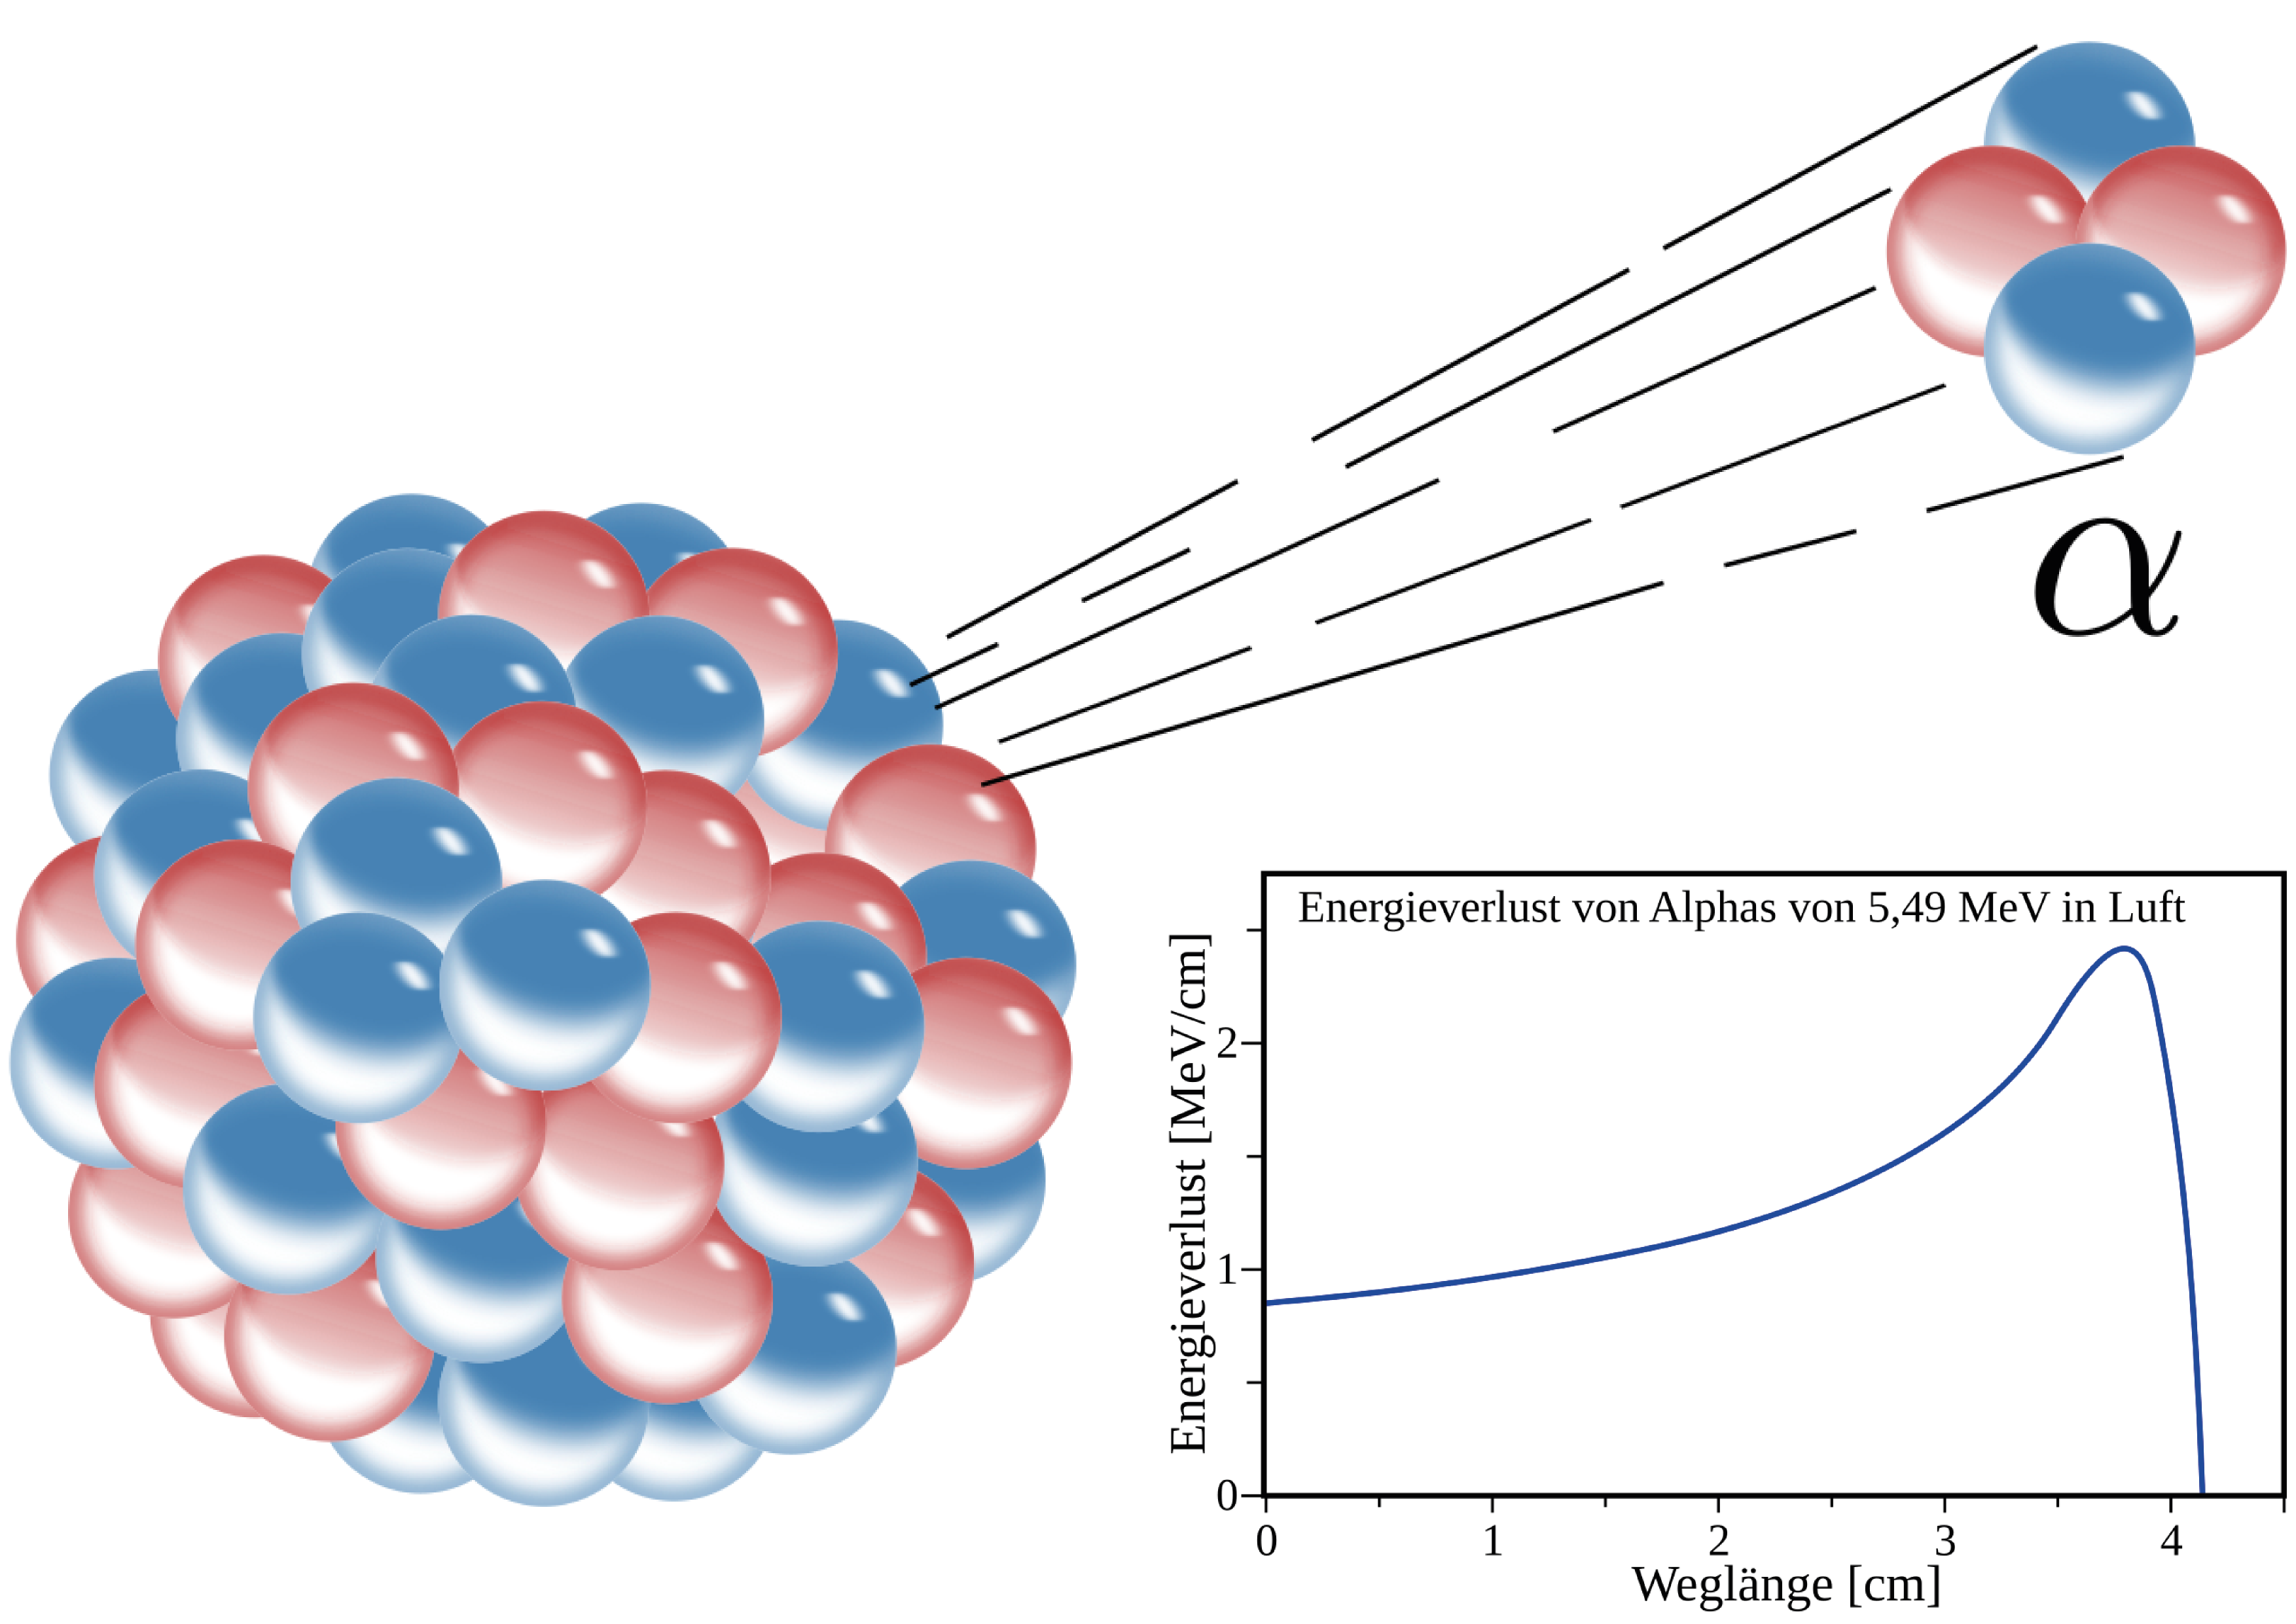
\includegraphics[width=14cm]{img/front_cover.png}
		\vfill
		{\Large\bfseries Fortgeschrittenen Praktikum} \\
		\vspace{0.3cm}
		{\Large at Institut für Kernphysik} \\
		\vspace{1.5cm}
		{\small 
			Dennis Spicker \& Beatriz Artur \\
			October 2024
		}
	\end{center} 
	\thispagestyle{empty}
	\clearpage
\end{titlepage}
%
\setcounter{tocdepth}{2}
\tableofcontents
\clearpage





% !TeX spellcheck = en_US
\section{Introduction}
When charged heavy particles (e.g. $\alpha$-particles or heavy ions) move through matter, they release their energy in the many collisions they make with the atoms. The more collisions they make, the slower they become and the greater the transferred energy. This phenomena is described by the so-called Bragg curve. At GSI Helmholtzzentrum für Schwerionenforschung in Darmstadt, for example, this feature is used in the field of medical research to irradiate tumors.

In this experiment, alpha radiation from a mixed source with three isotopes is measured with a surface barrier counter. The aim is to assess the radiation of the three isotopes by recording their energy spectra and determining the ranges and Bragg curves of the radiation. You will learn about alpha decay and gain an insight into the functioning of semiconductor detectors, the technical processing of signals and data analysis on the computer.

On the day of the lab course, you will be guided through the experiment by completing three tasks. Tasks 1 and 2 mainly deal with the characterization of the experimental set-up and Task 3 then examines how alpha radiation behaves in air.

\paragraph*{What you need to know to carry out the experiment:}
The necessary prior knowledge for this experiment covers three areas: the theory of alpha decay, the energy loss of charged particles in matter and how semiconductor detectors work. The topics are briefly introduced in the following subsections of section \ref{sec:theory}.

However, more knowledge is needed to carry out the experiment, which you should acquire yourself in a small literature search. Therefore, please carefully prepare beforehand the topics given at the end of each subsection. There are two books which are particularly recommended for this literature search: \textit{Particle Detectors: Fundamentals and Applications} \cite{kolanoski} and \textit{Particles and Nuclei} \cite{povh-rith}. Both are available as PDF files in the University library (as of January 2023).

After studying these topics, you should be able to answer the following questions, among others:
\begin{itemize}[itemsep=0pt]
	\item How are the $\alpha$-particles investigated in this experiment produced?
	\item Which feature of $\alpha$-particles can be measured with this experiment? 
	\item Does this feature have a constant value or is it different for each particle?
	\item How do the particles generate a signal in the semiconductor detector and how is the signal read out?
	\item What measured values (signal values) do you expect?
	\item What are the main sources of measurement inaccuracies?
	\item What is a histogram?
	\item What information is contained in the spectrum that is recorded on the computer?
	\item How do you obtain the observable you are looking for from the spectrum (e.g. energy loss per distance)?
	\item What happens when there is air in the apparatus?
\end{itemize}
%
\section{Theoretical Background}
\label{sec:theory}
%
\subsection{Alpha Decay}
$\alpha$-particles are identical to helium nuclei ($^4_2$He$^{2+}$), i.e. they consist of two protons and two neutrons. Their binding energy is high compared to nuclei of similar size and is approximately 7 MeV per nucleon. The typical kinetic energy of $\alpha$-particles which originate from natural decays of radioactive isotopes is in the range of $3-8$ MeV  \cite{povh-rith}. Further properties can be found in Table \ref{tab:alpha}.
\begin{table}[h]
	\centering
	\begin{tabular}{lc}
		Mass $m_\alpha$    & 3727.3 MeV$/c^{2}$ \\
		Mass number $A$        & 4    \\
		Atomic number $Z$   & 2    \\
		Binding energy $B$   & 28.3 MeV \\
	\end{tabular}
	\caption{Properties of $\alpha$-particles.}\label{tab:alpha}
\end{table}

Let $X$ denote the parent nuclide, $\Delta E$ its binding energy, $Y$ the daughter nuclide, $A$ the mass number and $Z$ the atomic number. Then the alpha decay process can be expressed as \cite{dewiki:240085809}:
\begin{equation*}
	^{A}_{Z}X \longrightarrow \ ^{A-4}_{Z-2}Y + \ ^4_2\text{He}^{2+} + \Delta E
\end{equation*}

Alpha decay releases a well-defined amount of energy in the form of kinetic energy, which corresponds to the binding energy of the system. This is possible thanks to the mass defect phenomena, in which the mass of a system is less than the sum of the masses of its constituents. 
In most alpha decays, the daughter nucleus goes directly to the ground state and the kinetic energy is taken solely by the $\alpha$-particle, creating a monoenergetic spectrum. However, decays to excited states of the daughter nucleus are also possible, in which the kinetic energy is thus shared between the two particles (although the $\alpha$-particle still keeps most of it) and the energy spectrum shows several monoenergetic lines, each corresponding to a decay to one of these states \cite{leo}. This spectrum is characteristic of the respective radionuclide and can therefore be used to determine it \cite{dewiki:240085809}.

Before the decay takes place, when the $\alpha$-particle is still inside the nucleus, it is attracted to it by the strong interaction, while also being electrically repelled by the protons in the nucleus. The strong nuclear force has a short range, while the weaker electrostatic repulsion has a long range. The potential therefore forms a kind of barrier, known as the Coulomb barrier, which is higher than the kinetic energy available to the $\alpha$-particle (see Fig. \ref{fig:coulomb-barrier}). According to classical physics, the $\alpha$-particle would therefore be stably bound in the nucleus; however, it can leave it by means of the quantum mechanical tunnel effect. The probability per time span for this can be very small and determines the half-life of the decay. The observed relationship between the half-life and the energy of the emitted $\alpha$-particles is described by the Geiger-Nuttall rule (see also the Gamow theory \cite{dewiki:240085809}.
\begin{figure}[h]
	\centering
	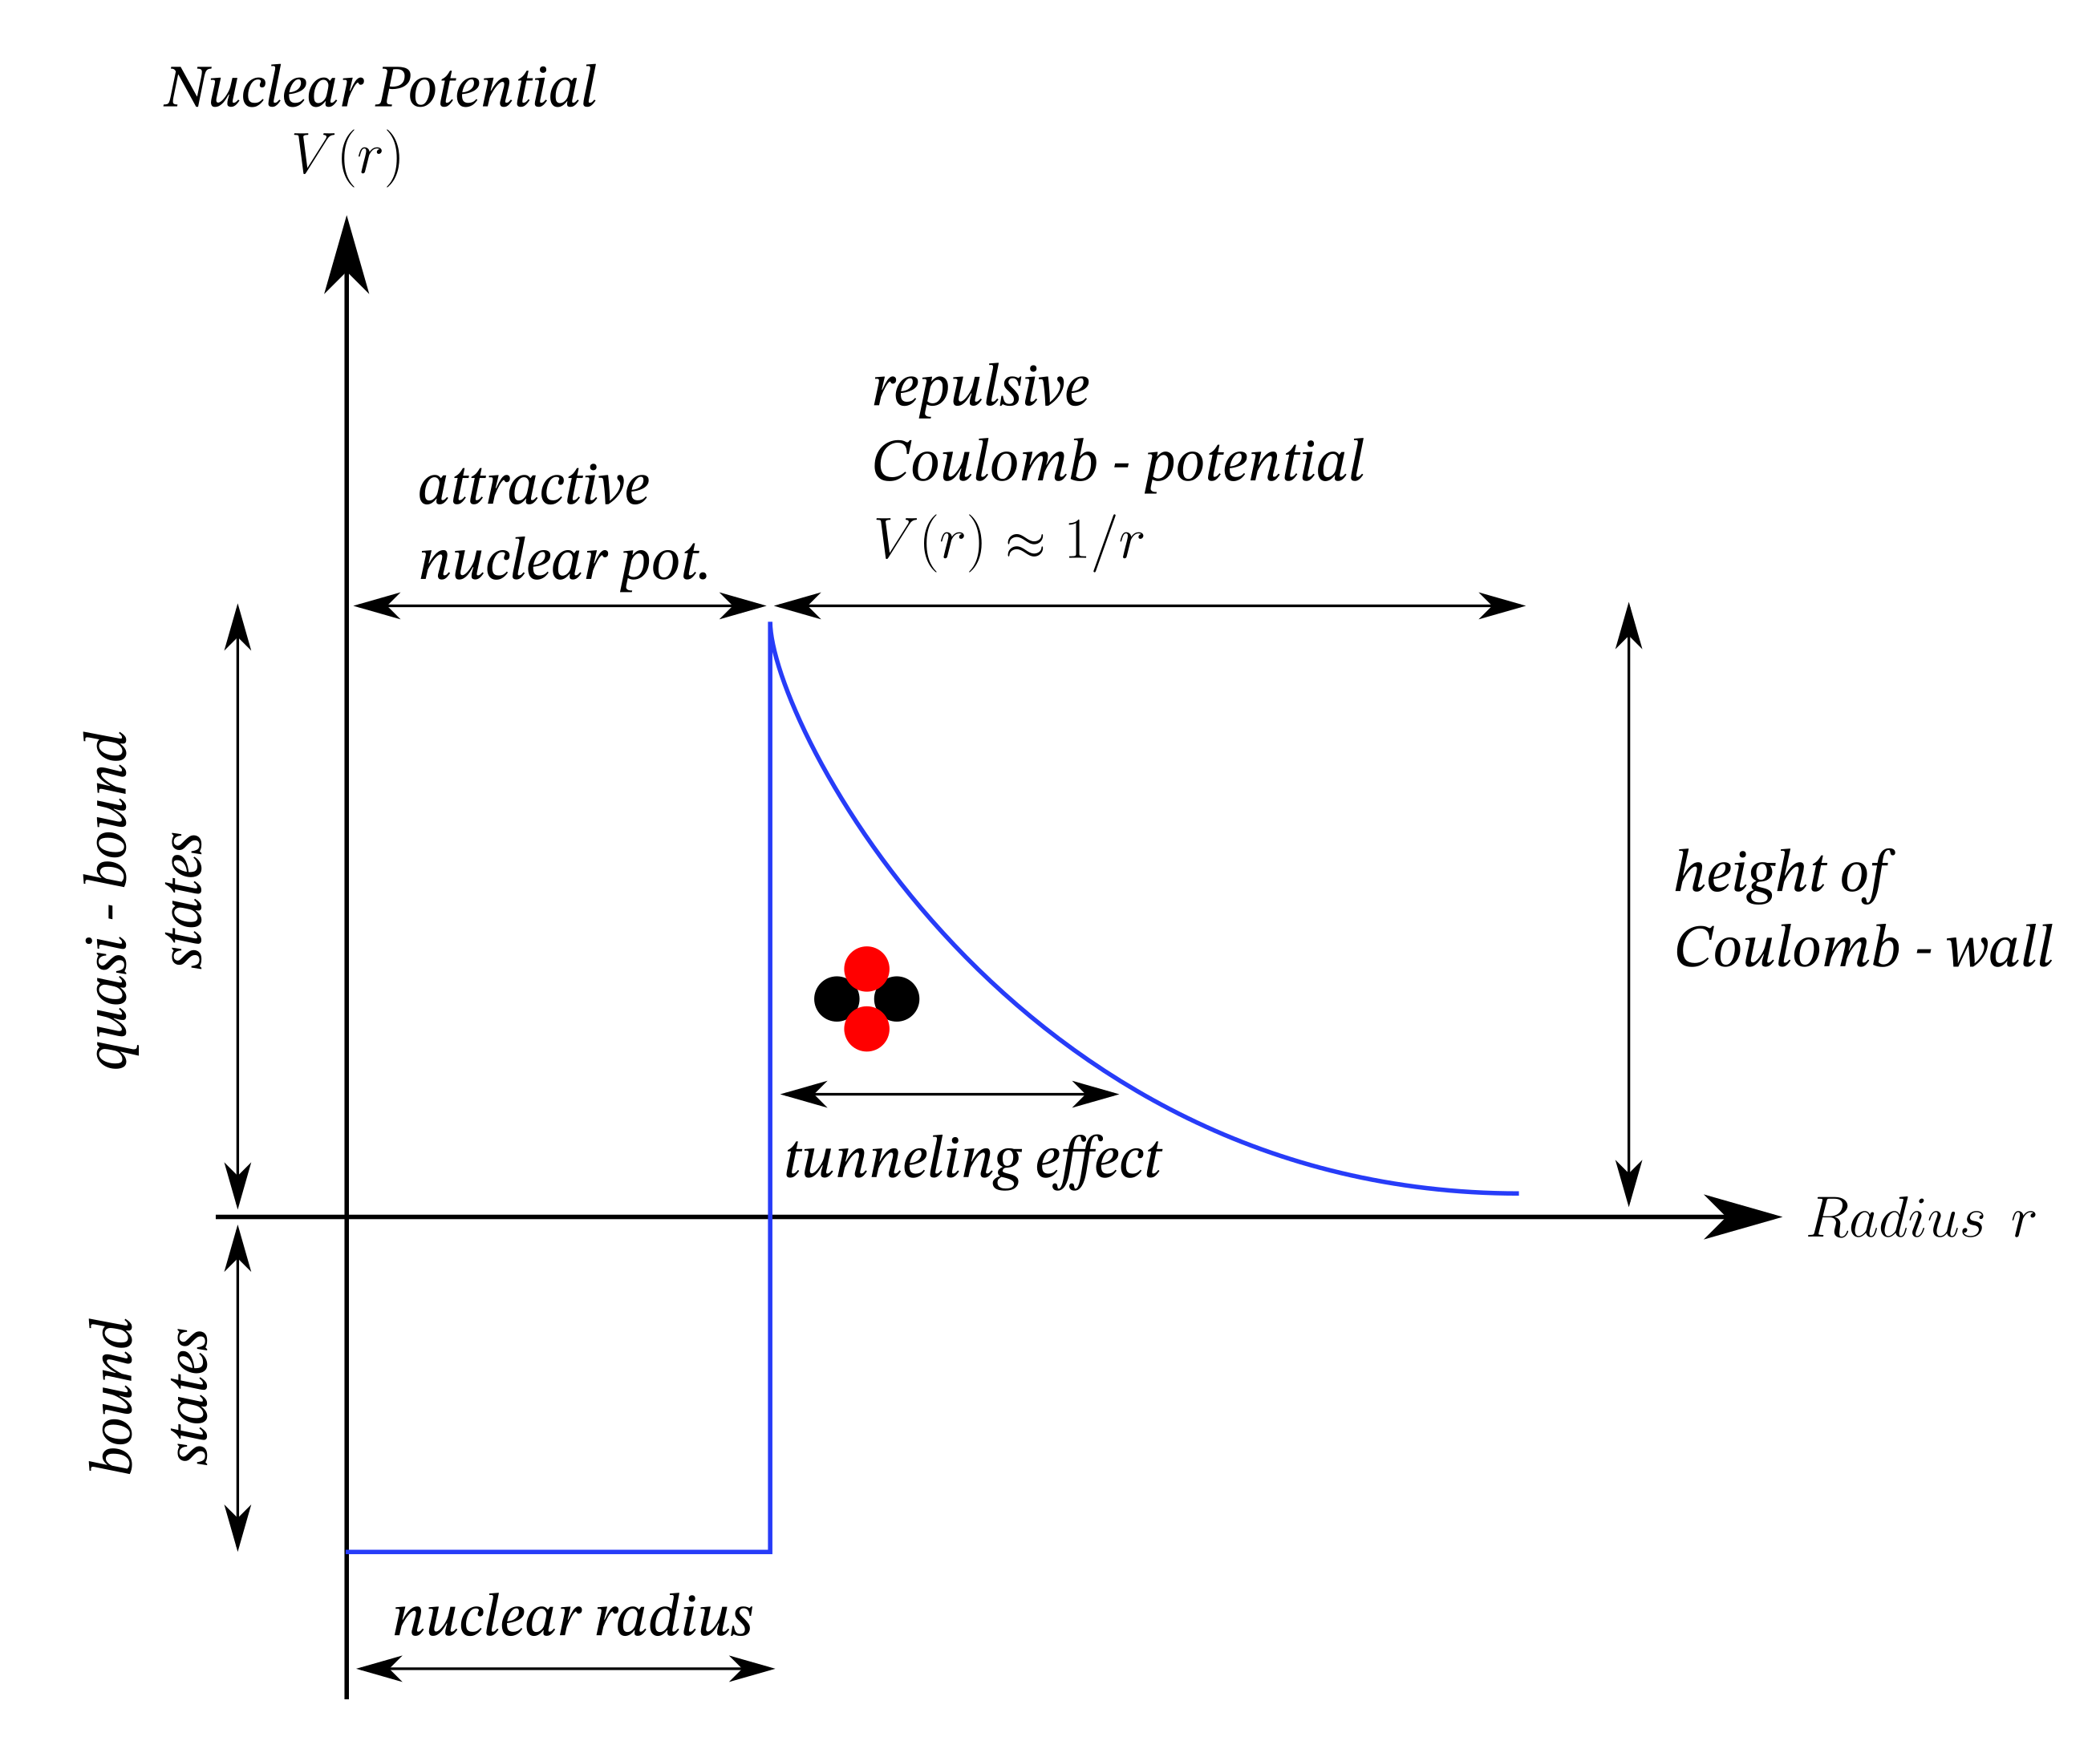
\includegraphics[width=0.6\linewidth]{img/tunneleffect_alpha_decay.png}
	\caption{Potential energy of the $\alpha$-particle $V(r)$ as a function of its distance to the center of the nucleus $r$. In the negative range ($V<0$), one sees the attractive potential caused by the strong nuclear force, and, in the positive range, the Coulomb barrier. \cite{img:coulombwall}}
	\label{fig:coulomb-barrier}
\end{figure}

In this experiment, the $\alpha$-particles are emitted from a mixed source composed of $^{239}$Pu, $^{241}$Am and $^{244}$Cm. Figure \ref{fig:spectrum} shows the measured decay spectrum of this mixed source. In addition to the main decay channels, one can see some extra secondary processes, which can be identified by the decay diagrams of Figure \ref{fig:schemata}.
\newpage
\paragraph{Topics for preparation}
\begin{itemize}
	\item Binding energy of atomic nuclei, mass defect
	\item Nuclide map, stability of nuclei
	\item Distance square law
	\item Line spectrum of alpha decay
	\item Properties of nucleons
	\item Gamow theory of alpha decay, Gamow factor, lifetime, potential of the atomic nucleus, tunnel effect
\end{itemize}

\begin{figure}
	\begin{center}
		%%\resizebox{0.8\textwidth}{!}{ \input{figs/Referenzmessung.tex} }
		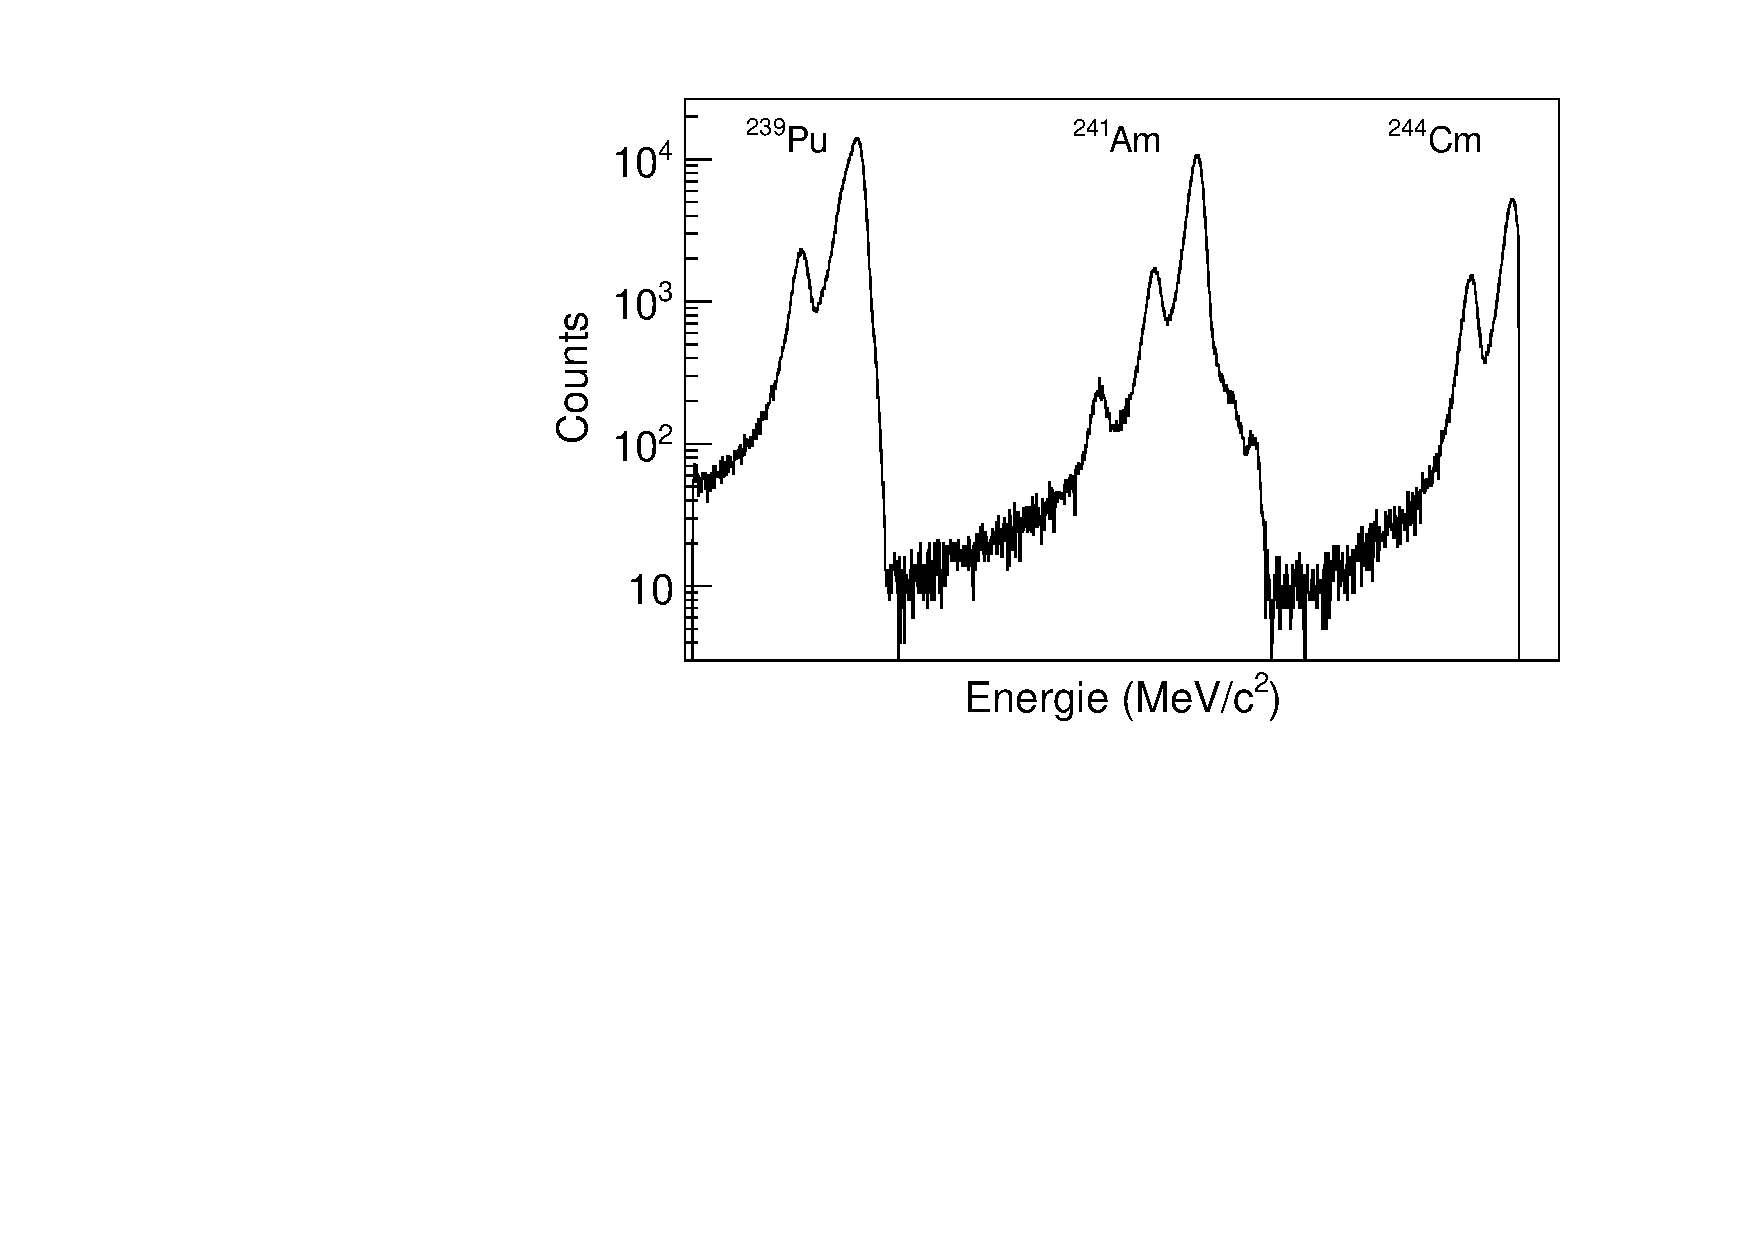
\includegraphics[width=0.9\linewidth]{img/Referenzmessung.pdf}
		\caption{Measured decay spectrum of the mixed source used in the experiment.}
		\label{fig:spectrum}
	\end{center}
\end{figure}
%
\begin{figure}
	\begin{center}
		\subcaptionbox{Plutonium}{ % I only need the arrows for this one.
%\usepackage{tikz}
%\usetikzlibrary{arrows}
% Place the TikZ picture in a figure environment.
%\begin{figure}
%\centerline{
  % Resize it to 5cm wide.
%\resizebox{horizontal length}{vertical length}{material}
  \resizebox{.3\linewidth}{!}{
    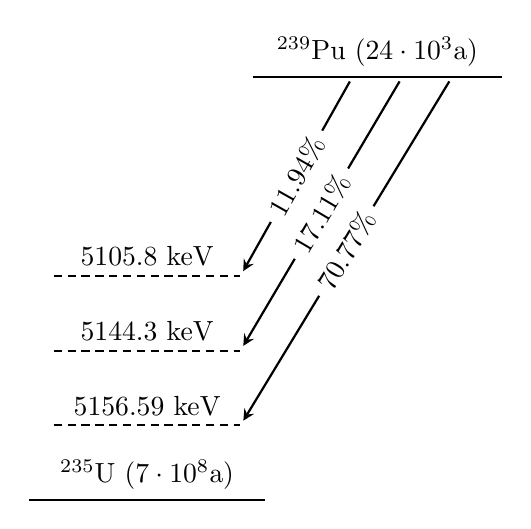
\begin{tikzpicture}[
      scale=0.45,
      level/.style={thick},
      virtual/.style={thick,densely dashed},
      trans/.style={thick,->,shorten >=2pt,shorten <=2pt,>=stealth},
      classical/.style={thin,double,<->,shorten >=4pt,shorten <=4pt,>=stealth}
    ]
    % Draw the energy levels.
    \draw[level] (20em,18em)    -- (40em,18em) node[midway,above] {$^{239}$Pu ($24\cdot10^3$a)};
    \draw[level] (2em,-16em)  -- (21em,-16em) node[midway,above] {$^{235}$U ($7\cdot10^8$a)};
    % Draw the virtual levels.
    \draw[virtual] (4em, 2em)  -- (19em, 2em)  node[midway,above] {5105.8 keV};
    \draw[virtual] (4em,-4em)  -- (19em, -4em)  node[midway,above] {5144.3 keV};
    \draw[virtual] (4em,-10em) -- (19em, -10em) node[midway,above] {5156.59 keV};
    % Draw the transitions.
    \draw[trans] (28em, 18em) -- node[sloped,fill=white] {$11.94\%$} (19em, 2em);
    \draw[trans] (32em, 18em) -- node[sloped,fill=white] {$17.11\%$} (19em, -4em);
    \draw[trans] (36em,18em) -- node[sloped,fill=white] {$70.77\%$} (19em,-10em);
    %    \draw[classical] (4.5cm,-8em) -- (1.5cm,-5em) node[midway,below] {\Ga{}};
    \end{tikzpicture}
  }
%}
%\caption{Zerfallschema}
%\end{figure}


%  \begin{comment}
%  http://www.nndc.bnl.gov/nudat2/decaysearchdirect.jsp?nuc=Pu239&unc=nds
%  
%  Author: E. BROWNE   Citation:Nuclear Data Sheets 98, 665 (2003)
%  
%  Half-Life: 24110 a
%  
%  Alphas:
%  
%  Energy (keV)	Intensity (%)	Dose ( MeV/Bq-s )
%  ...
%  ...
%    4529.6	     3.19E-6 % 3 	  1.445E-7 14 
%    4534	     2.84E-6 % 5 	  1.288E-7 23 
%    4559	     1.2E-5 % 5 	  5.5E-7 23 
%    4632 3 	     7.0E-4 % 20 	  3.2E-5 9 
%    4655	     2.8E-6 % 6 	  1.3E-7 3 
%    4691 3 	     5.0E-4 % 20 	  2.3E-5 9 
%    4718.5	     4.00E-5 % 10 	  1.89E-6 5 
%    4736 3 	     0.0051 % 8 	  2.4E-4 4 
%    4749 5 	     6.0E-4 % 6 	  2.8E-5 3 
%    4769 5 	     0.0015 % 6 	  7E-5 3 
%    4795 4 	     0.0012 % 6 	  6E-5 3 
%    4824	     2.30E-5 % 20 	  1.11E-6 10 
%    4828 3 	     0.0024 % 7 	  1.2E-4 3 
%    4866 5  ?	     0.0019 % 7 	  9E-5 3 
%    4871 5 	     7E-4 % 3 	  3.4E-5 15 
%    4912 5 	     0.0024 % 9 	  1.2E-4 4 
%    4934 3 	     0.0060 % 10 	  3.0E-4 5 
%    4960 5 	     0.0070 % 10 	  3.5E-4 5 
%    4987 3 	     0.0130 % 20 	  6.5E-4 10 
%    5006 5 	     0.0170 % 20 	  8.5E-4 10 
%    5028 3 	     0.009 % 3 	  4.5E-4 15 
%    5054 5 	     0.047 % 13 	  0.0024 7 
%    5076 5 	     0.078 % 8 	  0.0040 4 
%  *  5105.5 8 	    11.94 % 7 	  0.610 4 
%    5111 ?	     0.010 % 10 	  5E-4 5 
%  *  5144.3 8 	    17.11 % 14 	  0.880 7 
%  *  5156.59 14 	    70.77 % 14 	  3.649 7 
%    5156.7	     0.030 % 3 	  0.00155 15 
%  \end{comment}
 }
		\subcaptionbox{Americium}{ % I only need the arrows for this one.
%\usepackage{tikz}
%\usetikzlibrary{arrows}
% Place the TikZ picture in a figure environment.
%\begin{figure}
%\centerline{

% Resize it to 5cm wide.
  \resizebox{.3\linewidth}{!}{
  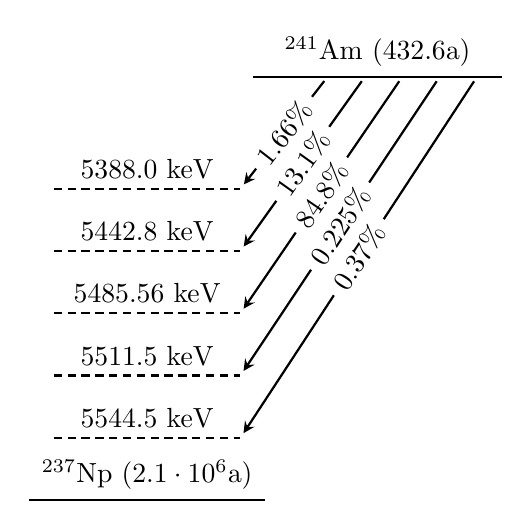
\begin{tikzpicture}[
      scale=0.45,
      level/.style={thick},
      virtual/.style={thick,densely dashed},
      trans/.style={thick,->,shorten >=2pt,shorten <=2pt,>=stealth},
      classical/.style={thin,double,<->,shorten >=4pt,shorten <=4pt,>=stealth}
    ]
    % Draw the energy levels.
    \draw[level] (20em,18em)    -- (40em,18em) node[midway,above] {$^{241}$Am (432.6a)};
    \draw[level] (2em,-16em)  -- (21em,-16em) node[midway,above] {$^{237}$Np ($2.1\cdot10^6$a)};
    % Draw the virtual levels.
    \draw[virtual] (4em,9em)  -- (19em,9em)  node[midway,above] {5388.0 keV};
    \draw[virtual] (4em,4em)  -- (19em,4em)  node[midway,above] {5442.8 keV};
    \draw[virtual] (4em,-1em) -- (19em,-1em) node[midway,above] {5485.56 keV};
    \draw[virtual] (4em,-6em) -- (19em,-6em) node[midway,above] {5511.5 keV};
    \draw[virtual] (4em,-11em) -- (19em,-11em) node[midway,above] {5544.5 keV};
    % Draw the transitions.
    \draw[trans] (26em, 18em) -- node[sloped,fill=white] {$1.66\%$}  (19em, 9em);
    \draw[trans] (29em, 18em) -- node[sloped,fill=white] {$13.1\%$} (19em, 4em);
    \draw[trans] (32em,18em) -- node[sloped,fill=white] {$84.8\%$}  (19em,-1em);
    \draw[trans] (35em,18em) -- node[sloped,fill=white] {$0.225\%$}  (19em,-6em);
    \draw[trans] (38em,18em) -- node[sloped,fill=white] {$0.37\%$}  (19em,-11em);
    %    \draw[classical] (4.5em,-8em) -- (1.5em,-5em) node[midway,below] {\Ga{}};
    \end{tikzpicture}
  }
%}
%\caption{Zerfallsschema Alphazerfalll von $^{241}$Am.}
%\end{figure}

%  http://www.nndc.bnl.gov/nudat2/decaysearchdirect.jsp?nuc=241AM&unc=nds
%  Author: M. S. Basunia   Citation:Nuclear Data Sheets 107, 3323 (2006)
%  Half-Life: 432.6
%  Alphas:
%  Energy (keV)   Intensity (%)   Dose ( MeV/Bq-s )
%    4758         5E-6 % 5    2.4E-7 24 
%    4800         8.6E-5 %   4.128E-6
%    4834         7E-4 %   3.384E-5
%    5004         1E-4 %   5.004E-6
%    5068         1.4E-4 %   7.0952E-6
%    5089         4.0E-4 % 4    2.04E-5 20 
%    5096         4.0E-4 % 4    2.04E-5 20 
%    5114         4E-4 %   2.0456E-5
%    5137         3.2E-4 %   1.644E-5
%    5155         7E-4 %   3.609E-5
%    5178         3E-4 %   1.553E-5
%    5182         9E-4 %   4.664E-5
%    5192         6E-4 %   3.115E-5
%    5217         1.0E-5 % 10    5E-7 5 
%    5223         0.0013 %   6.79E-5
%    5244         0.0024 %   1.259E-4
%    5279         5E-4 %   2.64E-5
%    5322         0.015 % 5    8E-4 3 
%  * 5388         1.660 % 20    0.0894 11 
%    5416.5       0.0100 % 10    5.4E-4 5 
%  * 5442.80 13   13.1 % 3    0.713 16 
%    5469         0.020 % 20    0.0011 11 
%  * 5485.56 12   84.8 % 5    4.65 3 
%  * 5511.5       0.225 % 5    0.0124 3 
%  * 5544.5  16   0.37 % 3    0.0205 17
 }
		\subcaptionbox{Curium}{ % I only need the arrows for this one.
%\usepackage{tikz}
%\usetikzlibrary{arrows}
% Place the TikZ picture in a figure environment.
%\begin{figure}
%\centerline{
  % Resize it to 5cm wide.
  \resizebox{.3\linewidth}{!}{
    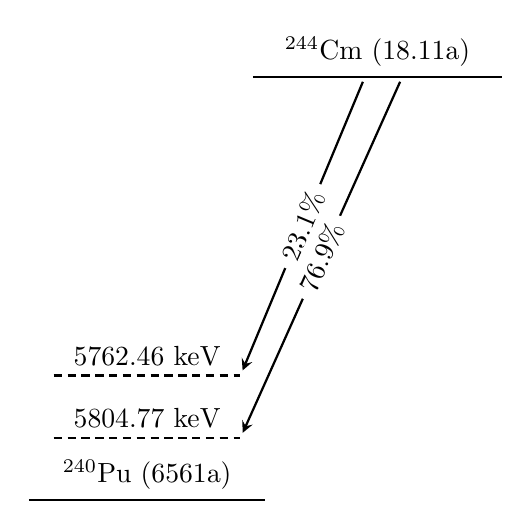
\begin{tikzpicture}[
      scale=0.45,
      level/.style={thick},
      virtual/.style={thick,densely dashed},
      trans/.style={thick,->,shorten >=2pt,shorten <=2pt,>=stealth},
      classical/.style={thin,double,<->,shorten >=4pt,shorten <=4pt,>=stealth}
    ]
    % Draw the energy levels.
    \draw[level] (20em,18em)   -- (40em,18em) node[midway,above] {$^{244}$Cm ($18.11$a)};
    \draw[level] (2em,-16em)  -- (21em,-16em) node[midway,above] {$^{240}$Pu ($6561$a)};
    % Draw the virtual levels.
    \draw[virtual] (4em,-6em)  -- (19em,-6em)  node[midway,above] {5762.46 keV};
    \draw[virtual] (4em,-11em)  -- (19em,-11em)  node[midway,above] {5804.77 keV};
    %    \draw[virtual] (0cm,-11em) -- (4cm,-11em) node[midway,above] {5.155 MeV};
    % Draw the transitions.
    \draw[trans] (29em, 18em) -- node[sloped,fill=white] {$23.1\%$} (19em, -6em);
    \draw[trans] (32em, 18em) -- node[sloped,fill=white] {$76.9\%$} (19em, -11em);
    %    \draw[classical] (4.5cm,-8em) -- (1.5cm,-5em) node[midway,below] {\Ga{}};
    \end{tikzpicture}
  }
%}
%\caption{Zerfallsschema}
%\end{figure}


%  Authors: BALRAJ SINGH, E. BROWNE   Citation:Nuclear Data Sheets 109,
%  2439 (2008)
%  
%  http://www.nndc.bnl.gov/nudat2/decaysearchdirect.jsp?nuc=244CM&unc=nds
%  
%  Half-Life: 18.11a
%  
%  Alphas:
%  
%  Energy 
%  (keV)	Intensity 
%  (%)	Dose 
%  ( MeV/Bq-s )
%    4920 3 	     5.0E-5 % 5 	  2.46E-6 25 
%    4960 3 	     1.49E-4 % 16 	  7.4E-6 8 
%    5166.64 7 	     4E-6 % 3 	  2.1E-7 15 
%    5215 3 	     5.6E-5 % 5 	  2.9E-6 3 
%    5315	     4E-5 %	  2.126E-6
%    5513 3 	     0.00352 % 18 	  1.94E-4 10 
%    5664 3 	     0.0204 % 15 	  0.00116 8 
%  *  5762.64 3 	    23.10 % 10 	  1.331 6 
%  *  5804.77 5 	    76.90 % 10 	  4.464 6 
%  

 }
		\caption{Decay diagrams of the alpha emitters: Pu~\cite{NDS2014}, Am~\cite{NDS2006} and Cm~\cite{NDS2008}.}
		\label{fig:schemata}
	\end{center}
\end{figure}
\FloatBarrier
%
\subsection{Interaction of charged particles in matter}
When passing through matter, $\alpha$-particles essentially lose their energy through ionization and excitation of the atoms in the material. As $\alpha$-particles are significantly more massive than the electrons of the material ($m_\alpha \approx 8000\ m_{e}$) with which they interact, they pass through the material without major deflections. The average energy loss per path length is described by the Bethe-Bloch formula \cite{kolanoski}. It depends on the properties of the medium as well as the charge and velocity of the particle.
\begin{equation}
	\left\langle - \frac{dE}{dx} \right\rangle = K \frac{Z}{A} \frac{z^2}{\beta^2} \ \left[ \frac{1}{2} \ln \left( \frac{2 m_e c^2 \beta^2 \gamma^2 T_{max}}{I^2} \right) - \beta^2 - \frac{\delta(\beta\gamma)}{2} \right] 
\end{equation}
\begin{itemize}[itemsep=0pt, label=-]
	\item $K=4\pi N_A r_e^2 m_e c^2 = 0.307\ \text{MeV cm}^2 / \text{mol} $ mit $r_e \approx 2.8$ fm;
	\item $z$ charge number, $\beta = v / c$ velocity of the projectile particle;
	\item $Z$ atomic number and $A$ mass number of the medium;
	\item $I$ average excitation potential of the atoms;
	\item $T_{max}$ maximum possible energy transfer to a shell electron, which is $\approx 2 m_e c^2 (\beta\gamma)^2$ in a central collision;
	\item $\delta$ density correction, which is important at high energies.
\end{itemize}

The Bethe-Bloch curve is shown in Figure \ref{fig:bethecurve}. For low particle velocities, the curve is approximately proportional to $1/\beta^2$. This means that the slower the particles become, the greater their energy loss per distance traveled. This results in the shape of the Bragg curve, which can be seen in Figure \ref{fig:braggpeak}.

Typically, $\alpha$-particles from nuclear decay have a kinetic energy of approximately 
$E_{kin} = 5$~MeV, i.e. a momentum of $p = \sqrt{2 \ m \ E_{kin} } = 195$~MeV$/c$ and it is $p/mc = 0.052$; they move at around $5\%$ of the speed of light.
This makes them considerably slower than e$^+$/e$^-$ from $\beta$ decays or neutron radiation, for example. 
%
\begin{figure}[h]
	\centering
	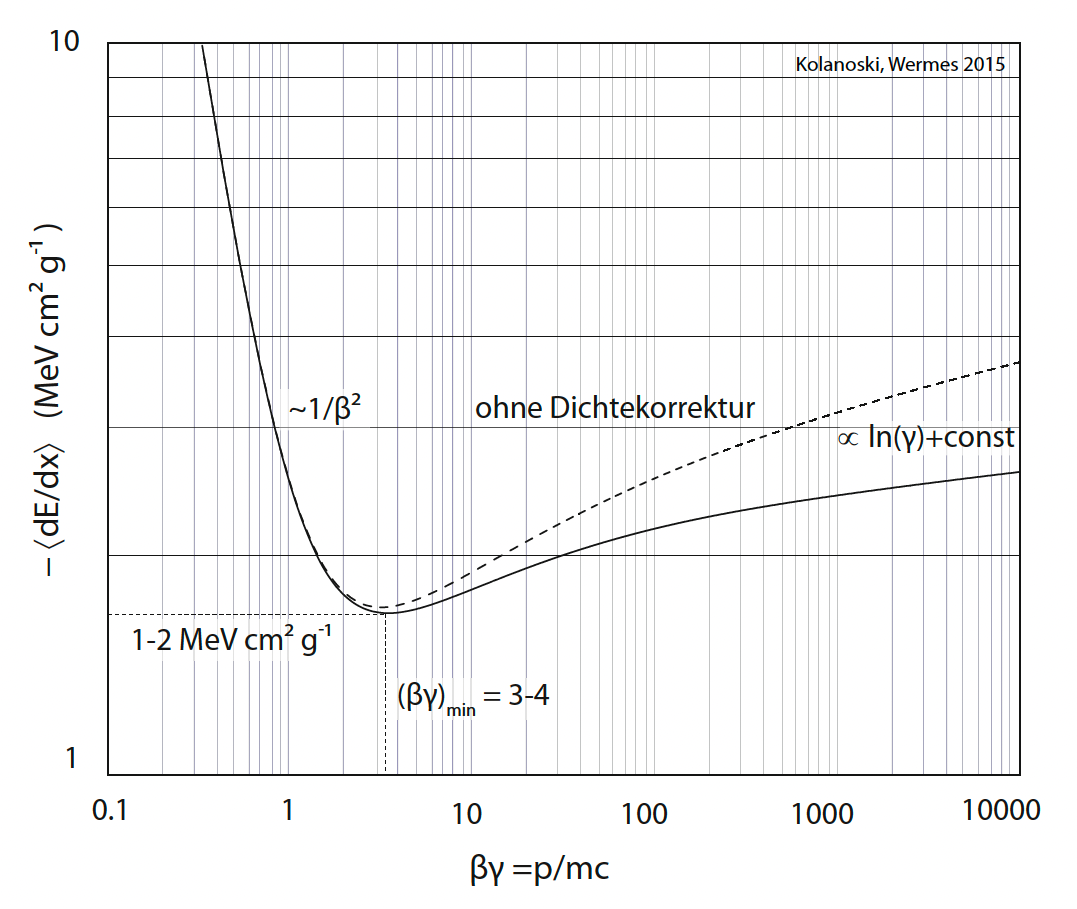
\includegraphics[width=0.7\linewidth]{img/bethe_curve.png}
	\caption{Average energy loss of charged particles in matter as a function of $p/mc$ \cite{kolanoski}.}
	\label{fig:bethecurve}
\end{figure}
%
\paragraph{Topics for preparation}
\begin{itemize}
	\item Energy loss of charged particles in matter
	\item Bethe-Bloch curve
	\item Bragg peak
	\item Radiation range and shielding
	\item Energy straggling
\end{itemize}
%
\begin{figure}[h]
	\centering
	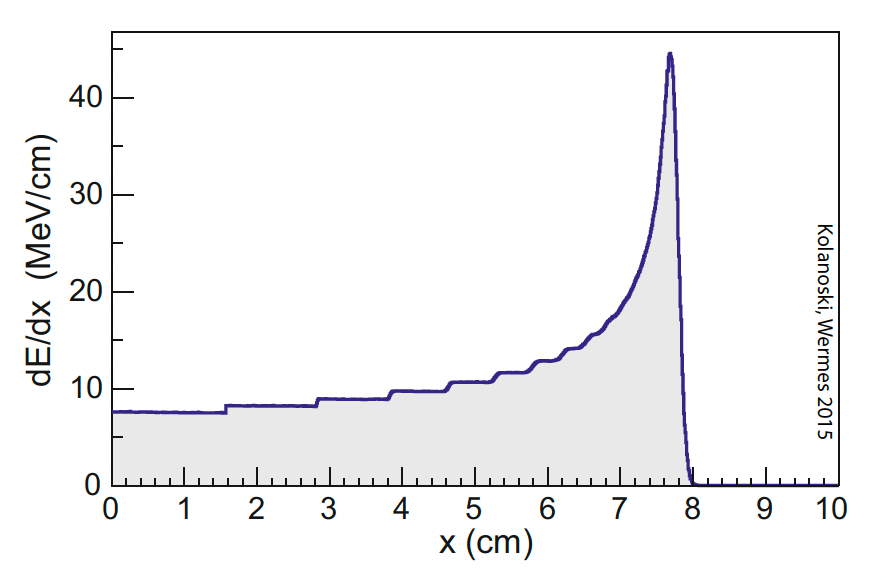
\includegraphics[width=0.7\linewidth]{img/bragg_peak.png}
	\caption{Energy loss per distance traveled as a function of the distance already traveled, for protons in water. One can see the Bragg peak. \cite{kolanoski}}
	\label{fig:braggpeak}
\end{figure}
\FloatBarrier
%
\subsection{Semiconductor detectors}
In principle, all particle detectors are suitable for detecting alpha radiation, for example for radiation protection purposes. However, the radiation must be able to reach the inside of the detector, i.e. the sensitive volume, and the counting tube must have a sufficiently thin foil window. For precise measurements, for example to determine the energy spectrum of the radiation, the radiation source and the detector must be in the same vacuum chamber. A semiconductor detector is usually used for this \cite{dewiki:240085809}.

Silicon semiconductor detectors are relatively large p-n semiconductor diodes with a very thin entrance window for charged particles, which offers minimal energy loss. They are operated in the reverse direction so that free charge carriers are sucked out of the sensitive volume (depletion zone) of the diode by an applied voltage. Figure \ref{fig:surfacebarrier} shows the structure of the detector used in this experiment. 

When a charged particle, such as an $\alpha$-particle, enters the detector, it loses a small part of its energy at the thin entrance window. The majority of its energy is deposited in the depletion zone by ionization of the silicon atoms. The number of electron-hole pairs generated by this process is proportional to the energy of the incoming particle. The free charge generated by the ionization is extracted from the electrodes and collected by the capacitors of the preamplifier connected via the connector. The collected charge results in a voltage pulse, which is determined by the capacitance of the preamplifier and the amount of charge and rises within up to $100$~ns. The amplitude of the voltage pulse is proportional to the energy of the measured $\alpha$-particle and can be further processed for evaluation using a multichannel pulse height analyzer (MCA).

%
\begin{figure}[h]
	\centering
	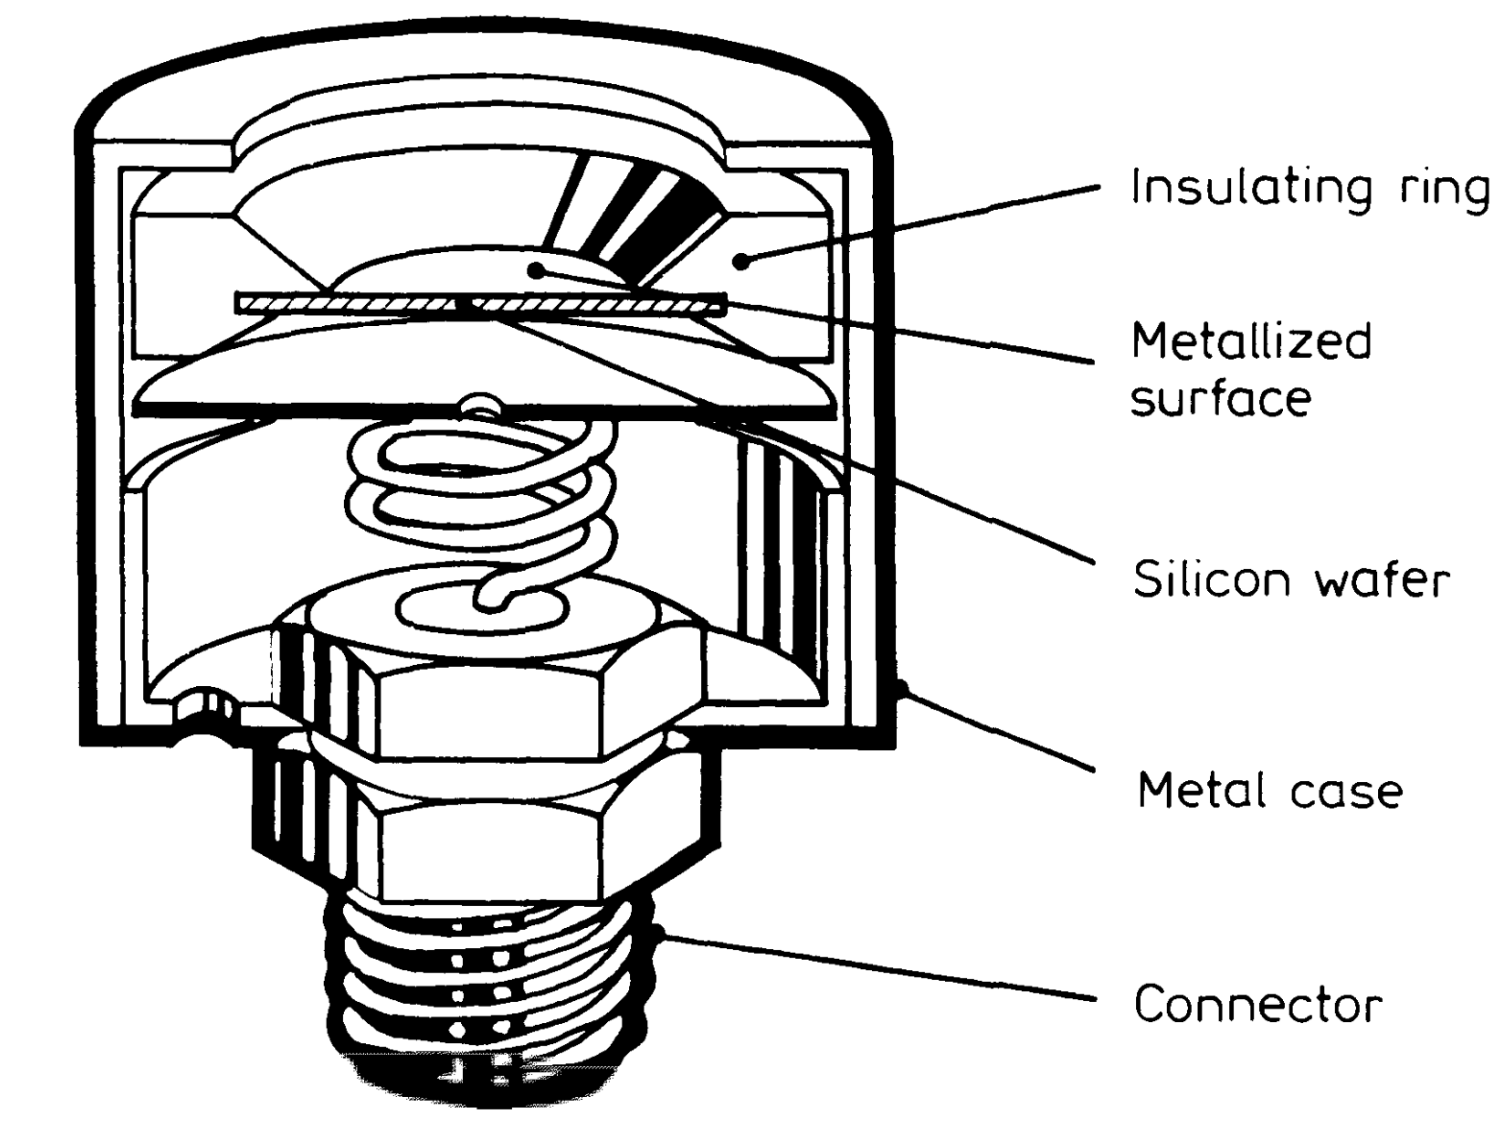
\includegraphics[width=0.7\linewidth]{img/surface.png}
	\caption{Structure of the surface barrier layer counter \cite{leo}.}
	\label{fig:surfacebarrier}
\end{figure}

\hfill
\hfill

Semiconductor detectors can be used in a wide energy range, namely for electrons with about 20 keV up to heavy ions with 200 MeV. Their efficiency in the active volume is close to $100\%$, while the proportionality of charged particle energy to pulse height is constant over a wide range. In this experiment, a silicon semiconductor detector will be used for $\alpha$-particle spectroscopy.
\paragraph{Topics for preparation}
\begin{itemize}
	\item Semiconductors, doping, diode, p-n junction, diffusion voltage
	\item Energy deposition, formation and recombination of charge carriers
	\item Energy resolution of the semiconductor detector
	\item Thermal noise, energy per electron-hole pair
	\item Poisson statistics, Fano factor (see \cite[Kap. 17.10.2]{kolanoski})
\end{itemize}

% !TeX spellcheck = en_US
\clearpage
\section{Experimental Setup}
The experimental setup consists of the following components:
\begin{itemize}
	\item Radiation source
	\item Semiconductor detector
	\item Vacuum container with pressure gauge, \\inlet (to let the air in) and outlet (for vacuum) valves
	\item Vacuum pump
	\item Preamplifier and main amplifier
	\item Power supply unit with external voltage measuring device
	\item Multi-channel pulse height analyzer (MCA) inside the PC
	\item PC with MCA software
\end{itemize}

Figure \ref{fig:aufbauhalbleiter} shows the experimental setup schematically, while photographs of the actual experiment are shown in Figure \ref{fig:setup_}. The surface barrier counter and the alpha radiation source are located in an airtight metal cylinder. The source can be moved in the cylinder along one spatial axis in order to change the distance between the source and detector. At the minimum adjustable distance, the source does not touch the detector. In fact, determining this minimum distance is part of the experiment.
\begin{figure}[h]
	\centering
	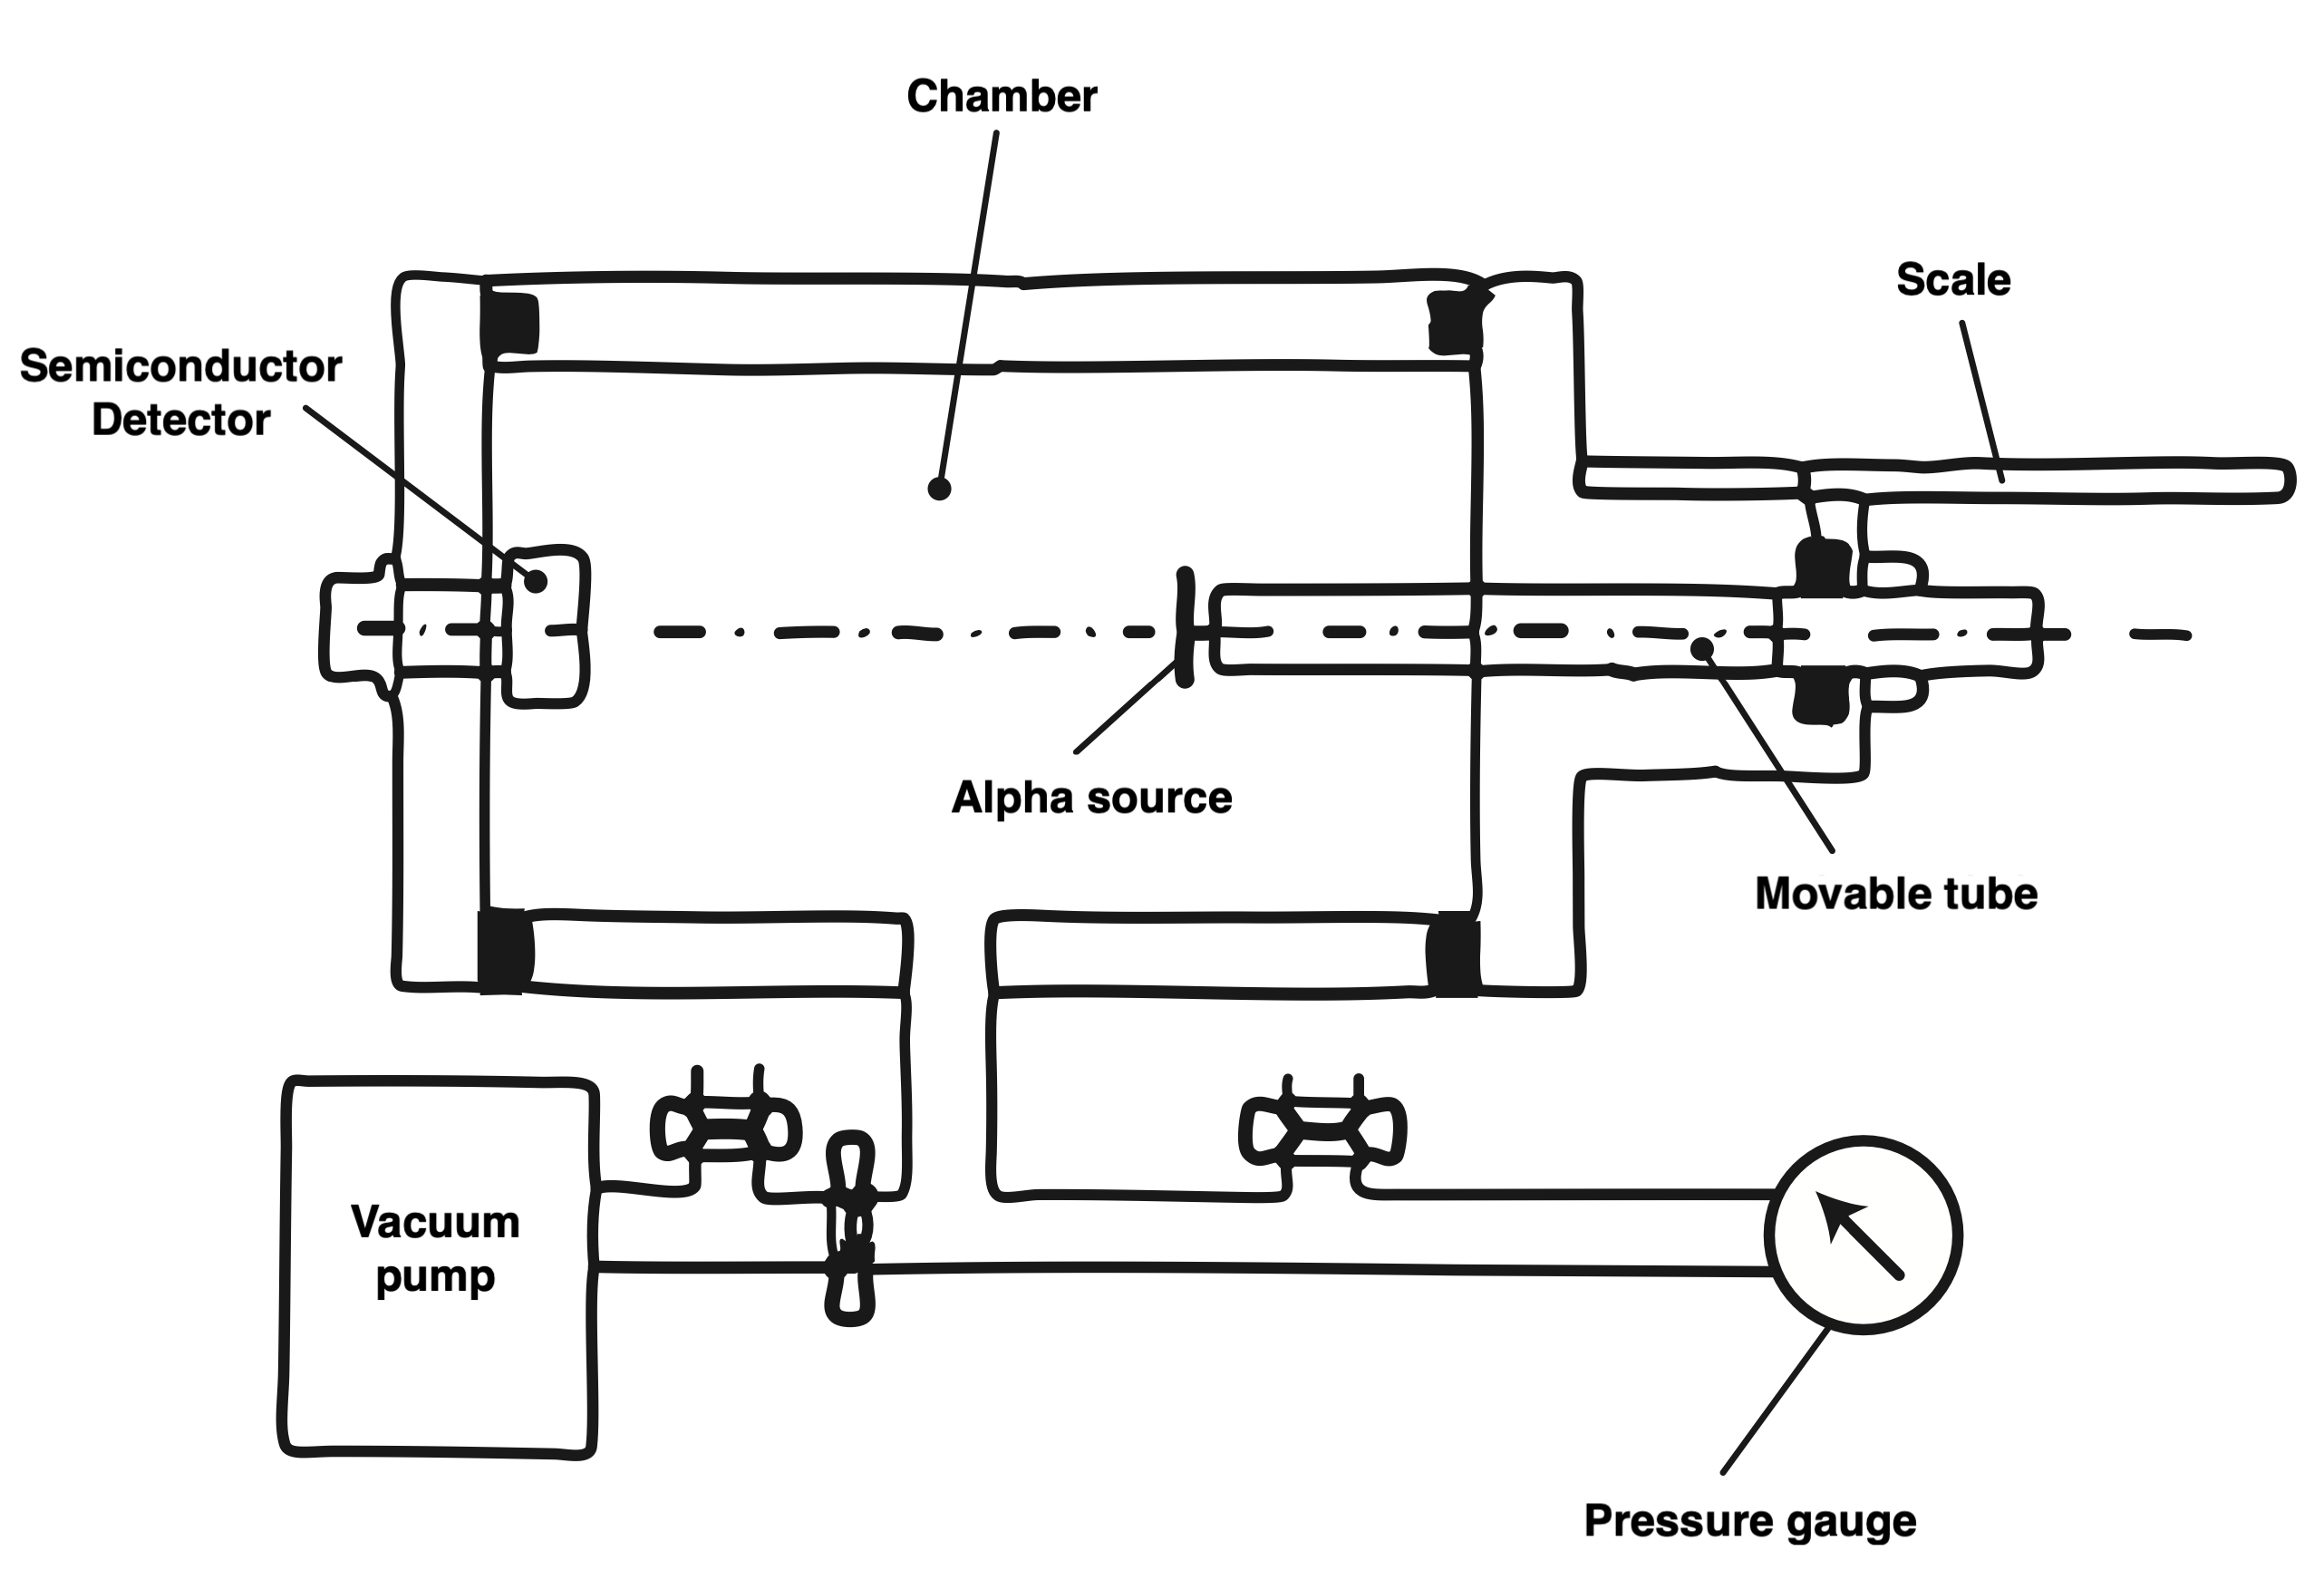
\includegraphics[width=0.7\linewidth]{img/schematics_exp.png}
	\caption{Schematics of the experimental setup.}
	\label{fig:aufbauhalbleiter}
\end{figure}

\hfill

The mixed source has an active area with a diameter of about 7~mm and is covered by a gold  layer, which is about 2~\textmu m thick (see Figure \ref{fig:quellefoto}). However, the covering of the radioactive material does not provide protection against contamination on contact. Hence, the source must be considered open and special licensing requirements and precautions must be taken into account (see section \ref{sec:warningnotices}).
The preamplifier is attached to the semiconductor detector directly outside the vacuum container. The entrance window of the detector can be seen in Figure \ref{fig:detektorfoto}. The preamplifier has several connections: 
\begin{itemize}[itemsep=0pt]
	\item Operating voltage supply, connected to the rear of the main amplifier.
	\item Signal output, connected to signal input of the main amplifier.
	\item External voltage input, connected to the power supply unit.
	\item Connection option for a pulser. Not connected.
\end{itemize}
The wiring of the experiment is shown in figure \ref{fig:verkabelung} and figure \ref{fig:setup3} shows a picture of the main amplifier as well as the voltage supply unit.
\begin{figure}[h]
	\centering
	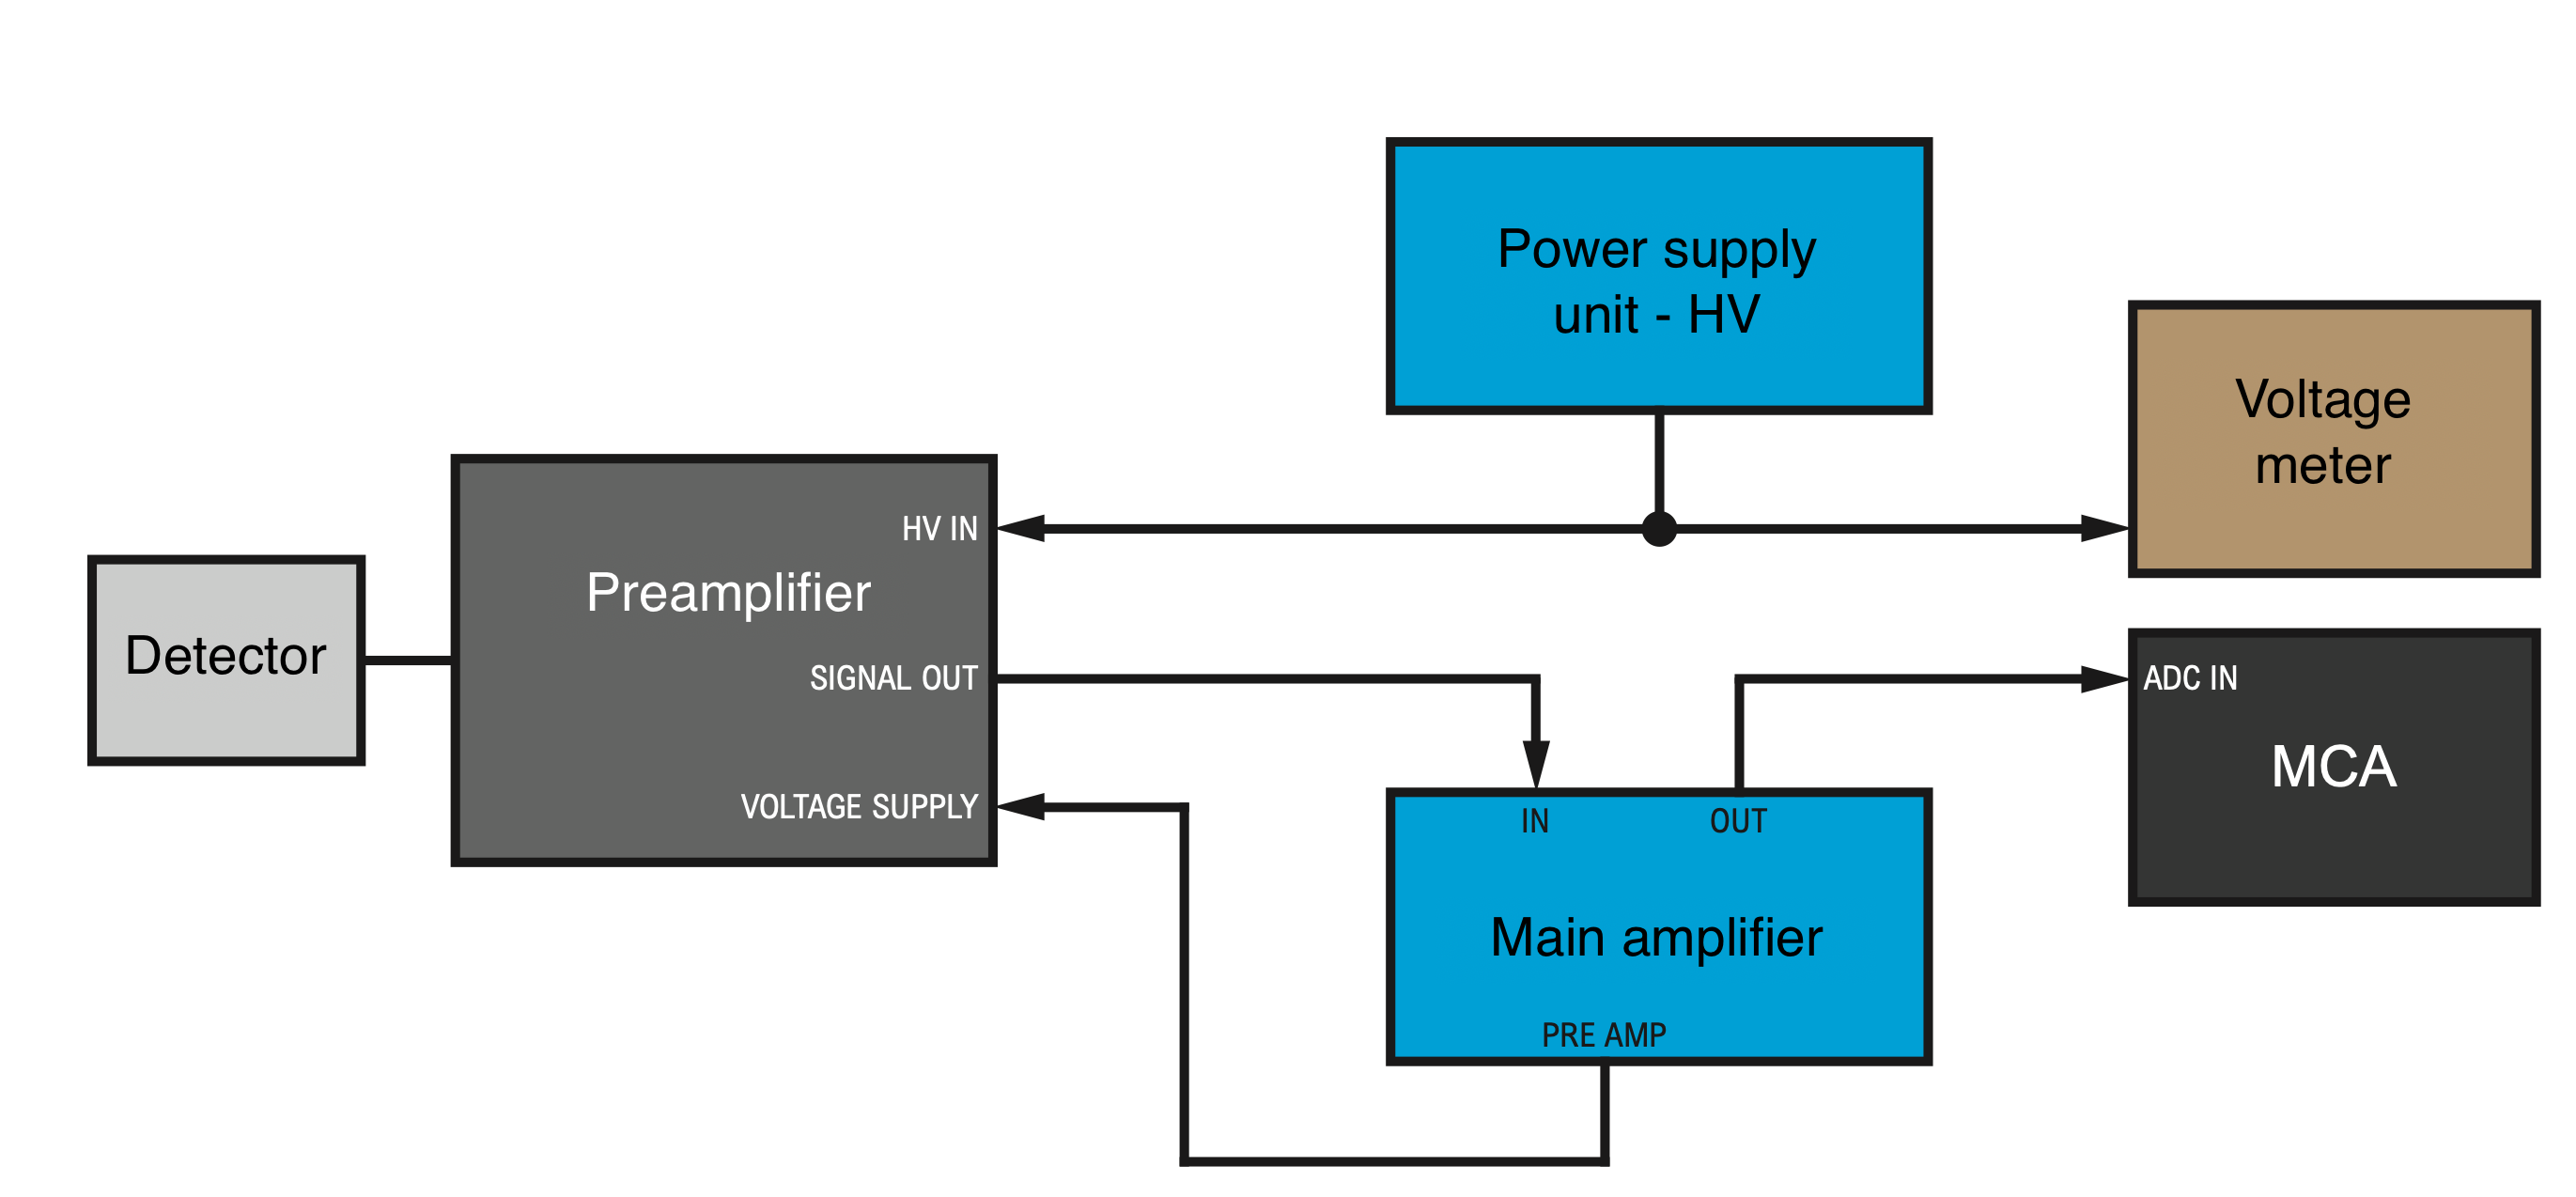
\includegraphics[width=\linewidth]{img/wiring.png}
	\caption{Schematics of the wiring of the experiment.}
	\label{fig:verkabelung}
\end{figure}

\begin{figure}
	\centering
	\subcaptionbox{View from the left. \label{fig:setup1}}[.49\linewidth]{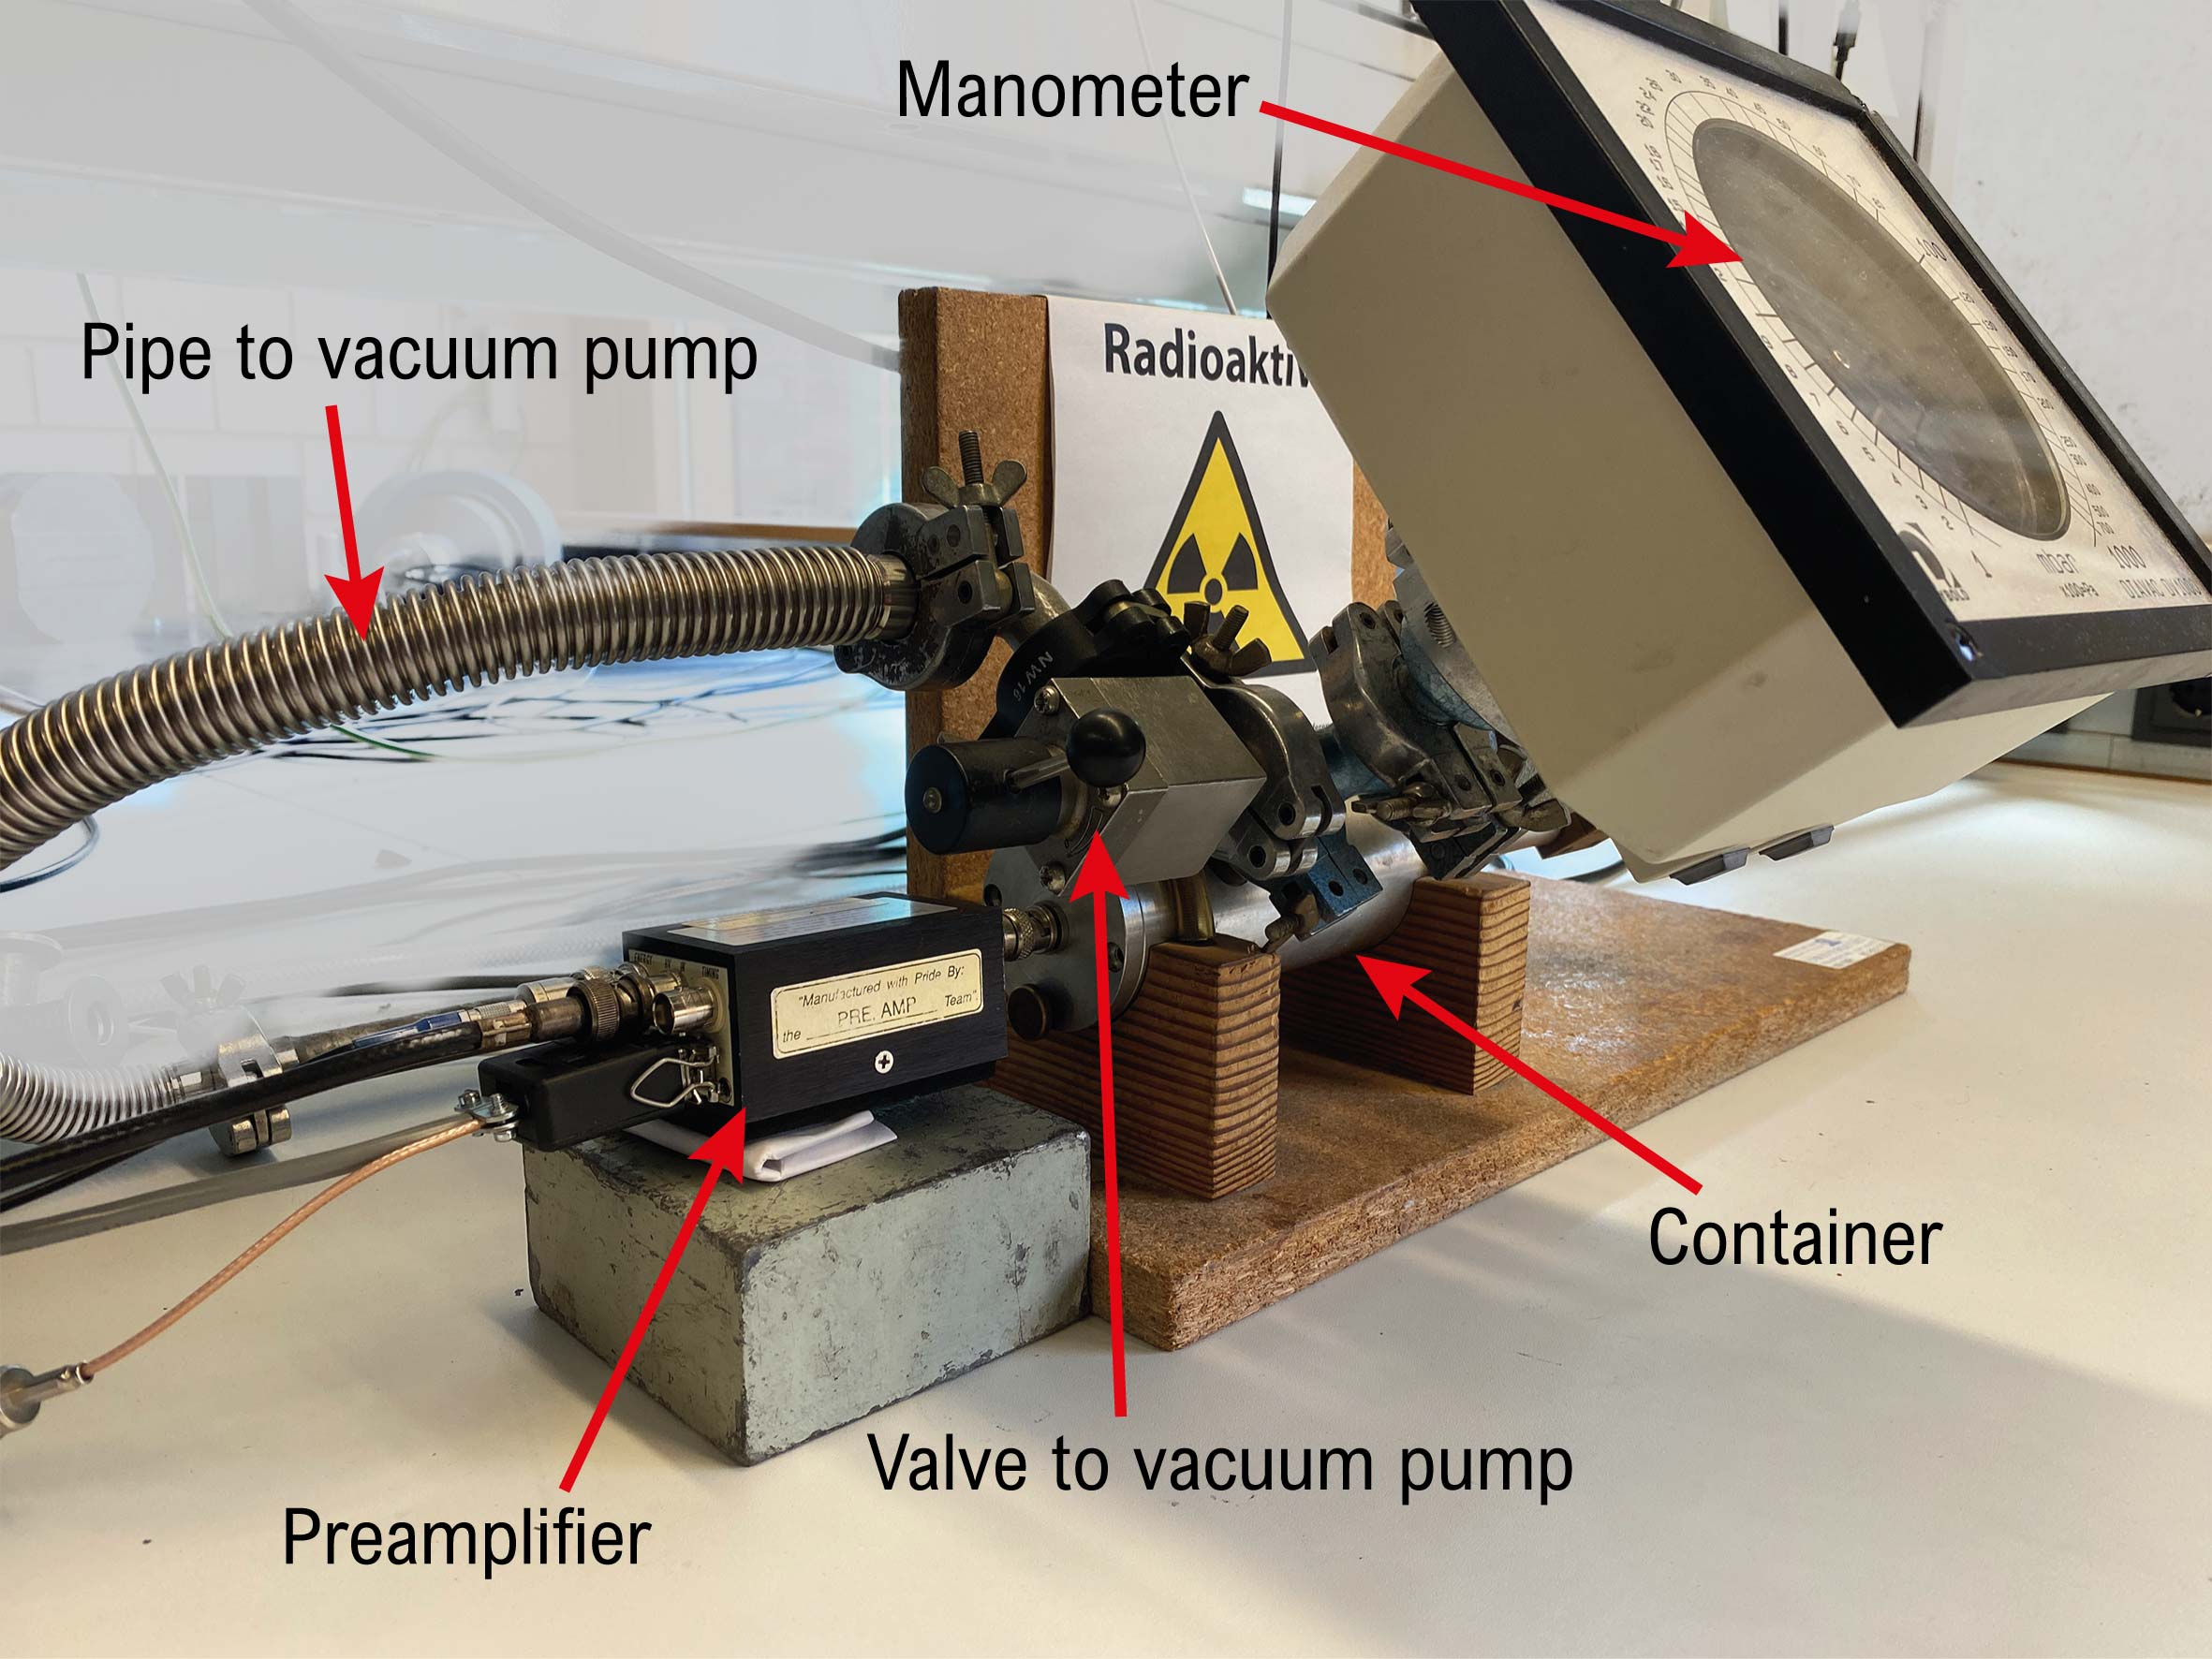
\includegraphics[width=\linewidth]{img/setup_1.jpg}}
	\subcaptionbox{View from the right. \label{fig:setup2}}[.49\linewidth]{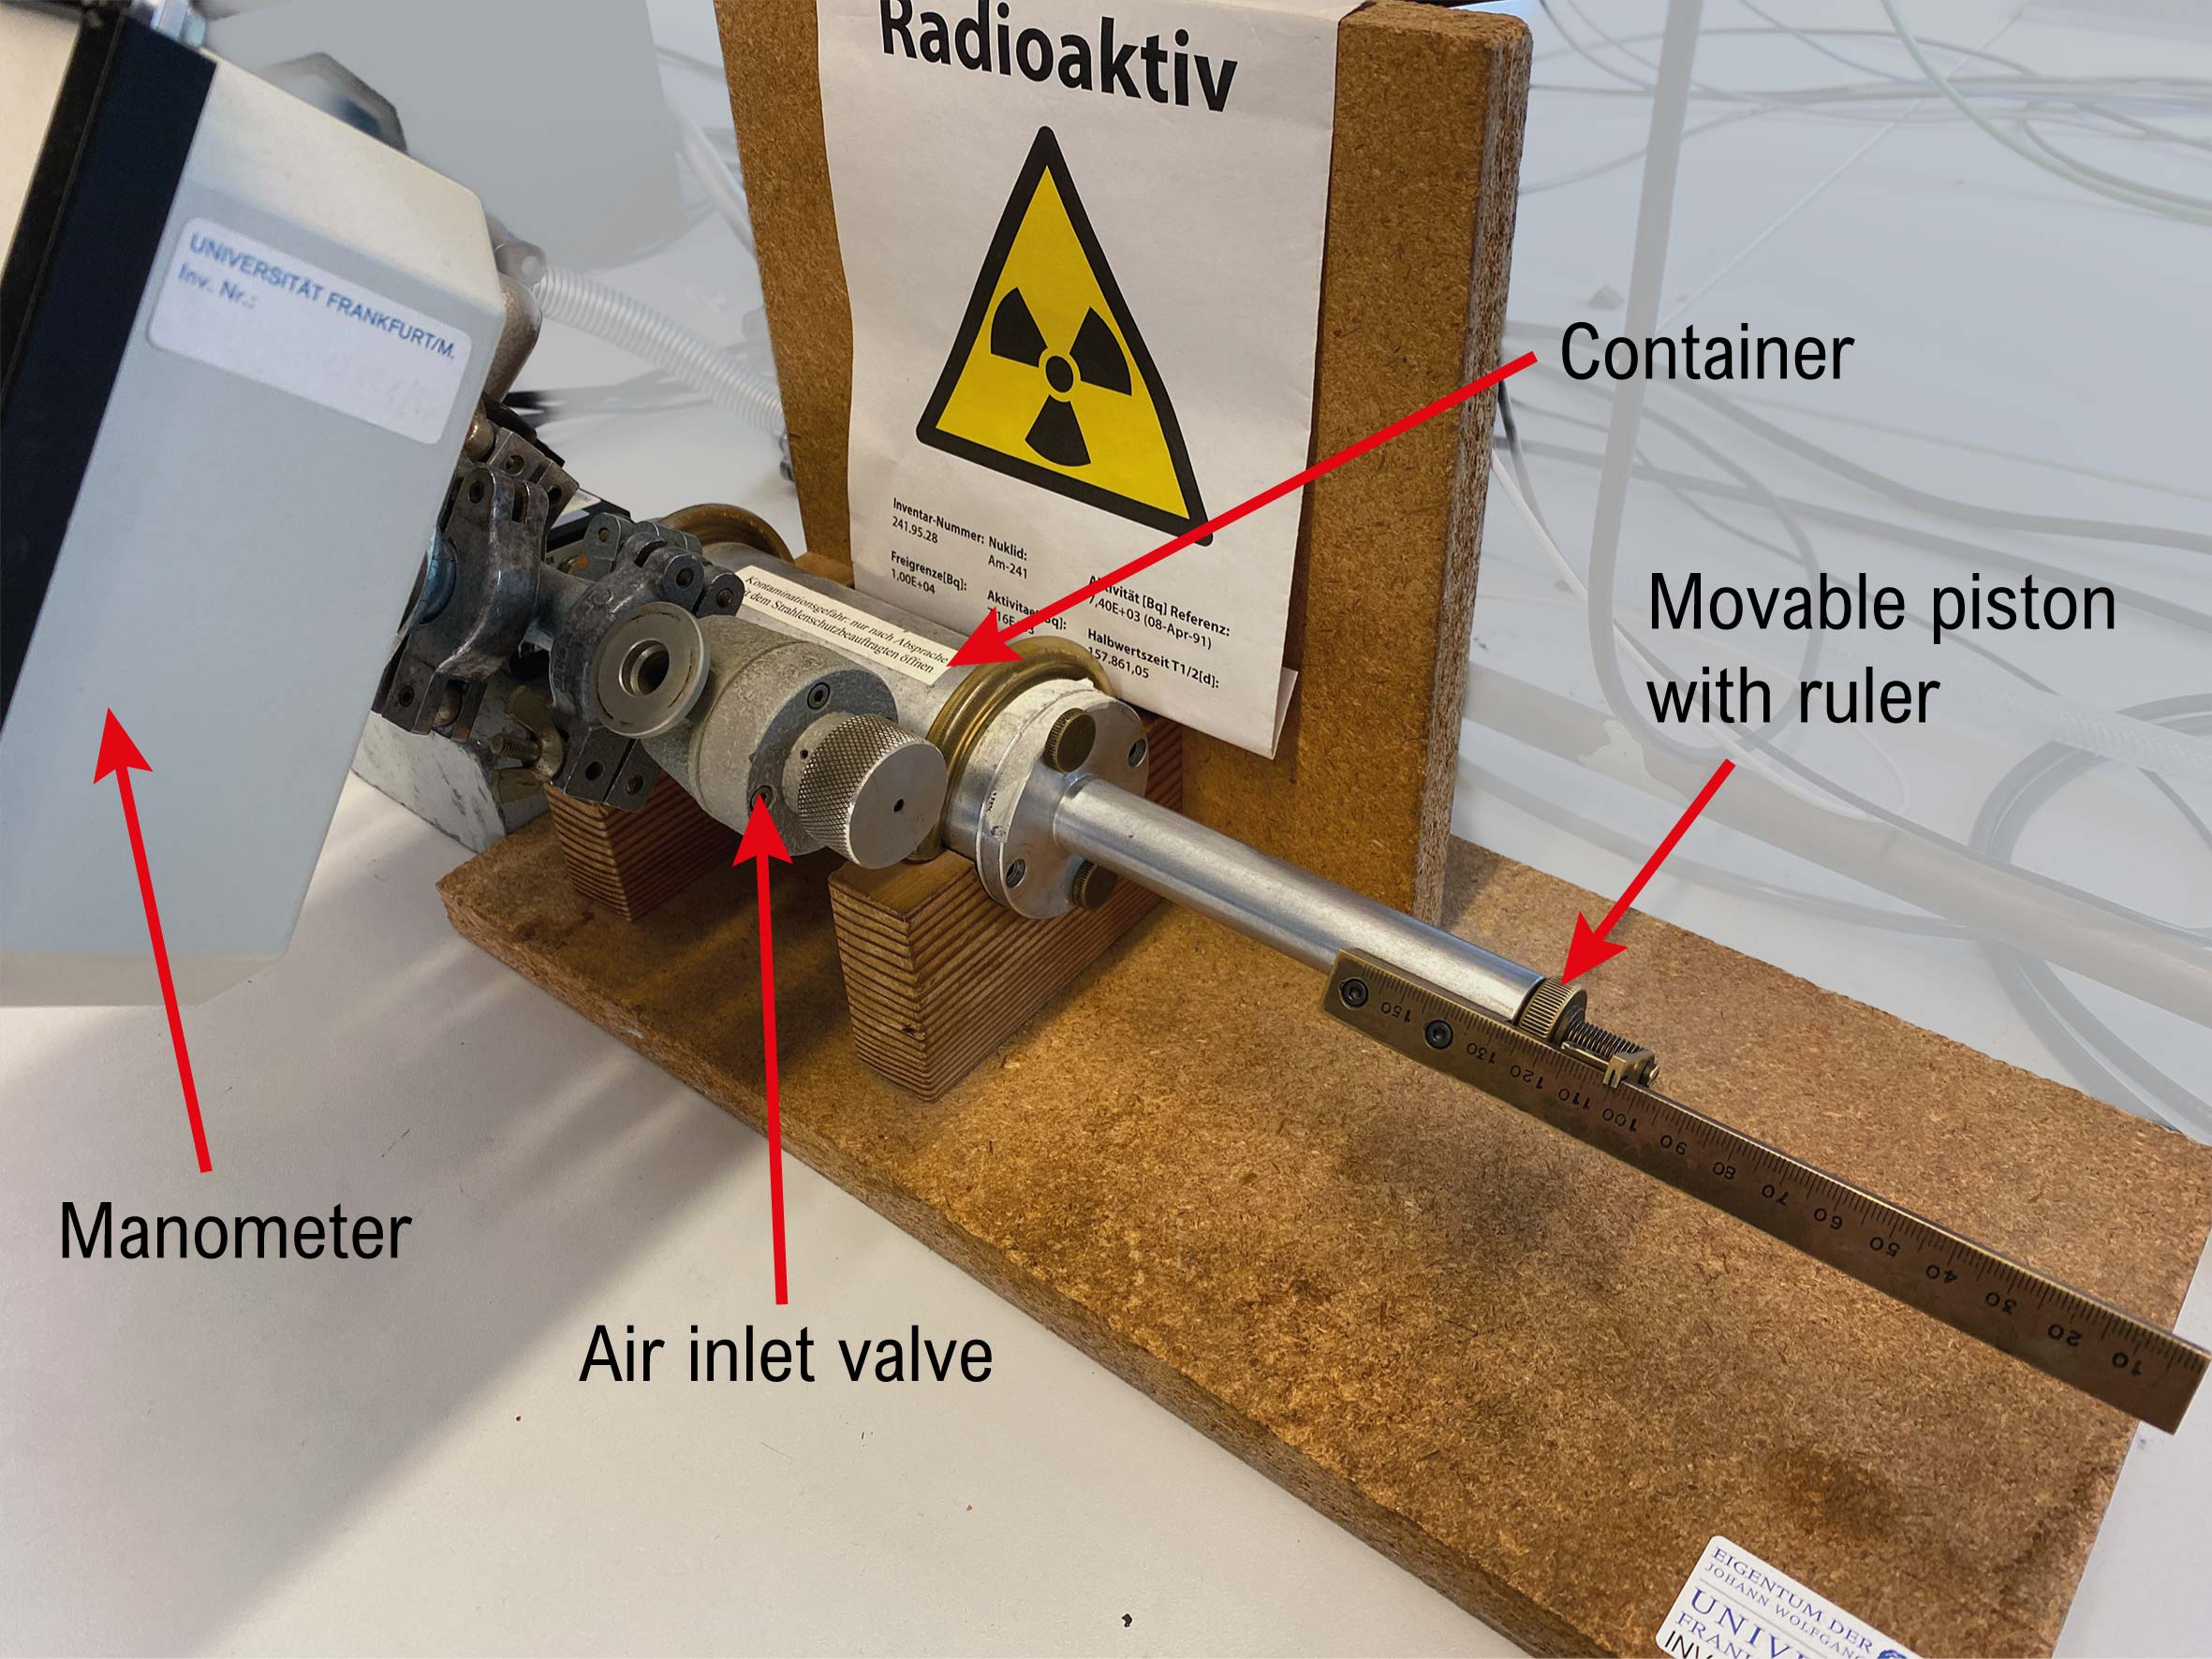
\includegraphics[width=\linewidth]{img/setup_2.jpg}}
	\caption{The experimental setup.}
	\label{fig:setup_}
\end{figure}
\begin{figure}
	\centering
	\subcaptionbox{The semiconductor detector. \label{fig:detektorfoto}}[.49\linewidth]
	{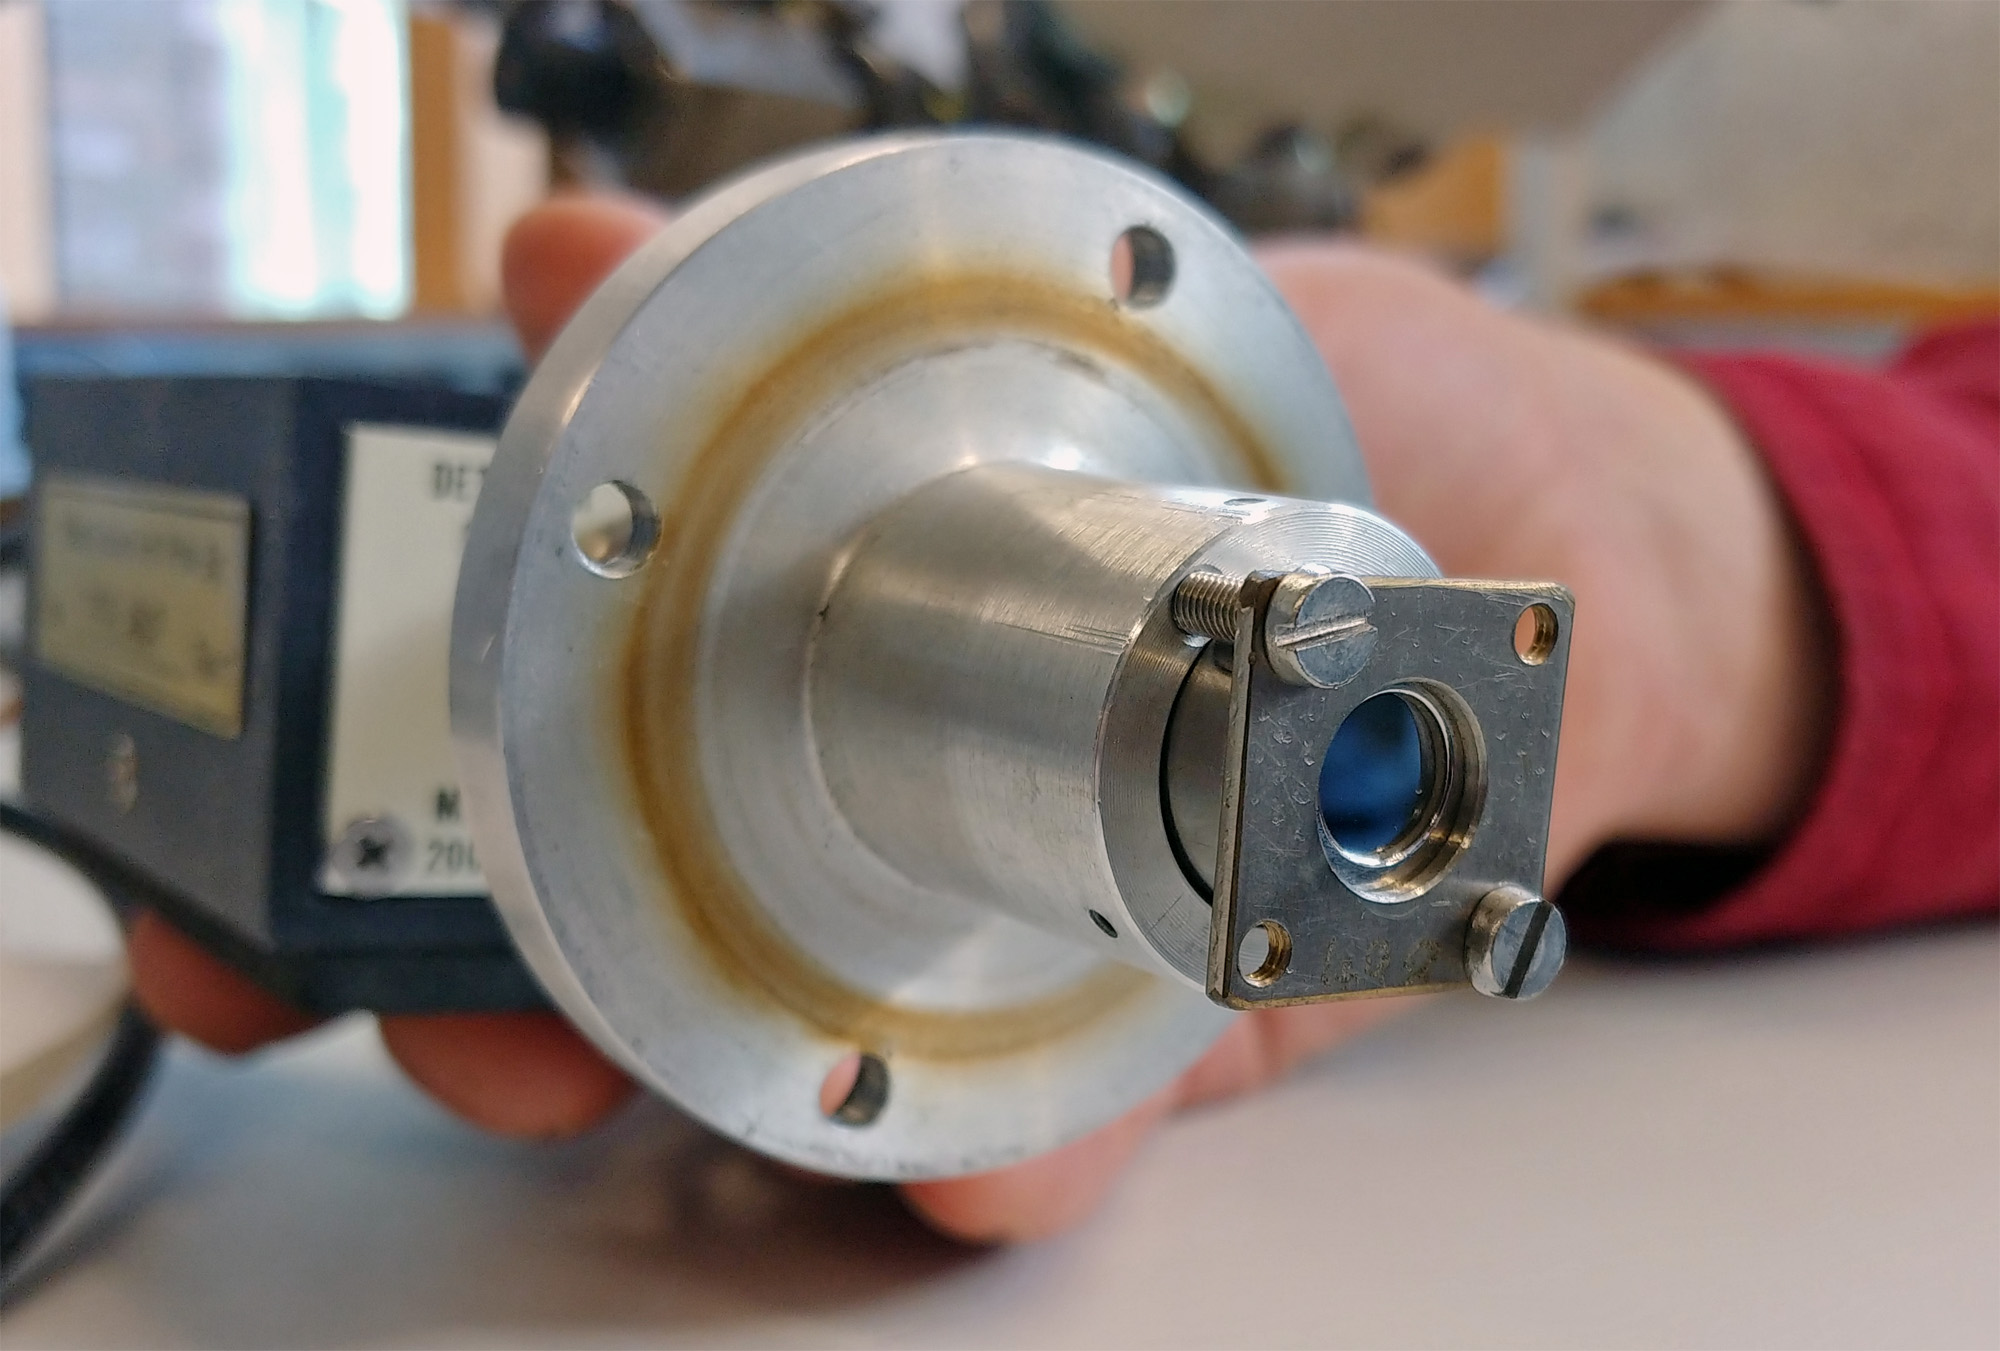
\includegraphics[width=\linewidth]{img/detektor_foto}}
	\subcaptionbox{The radiation source with golden surface. \label{fig:quellefoto}}[.49\linewidth]
	{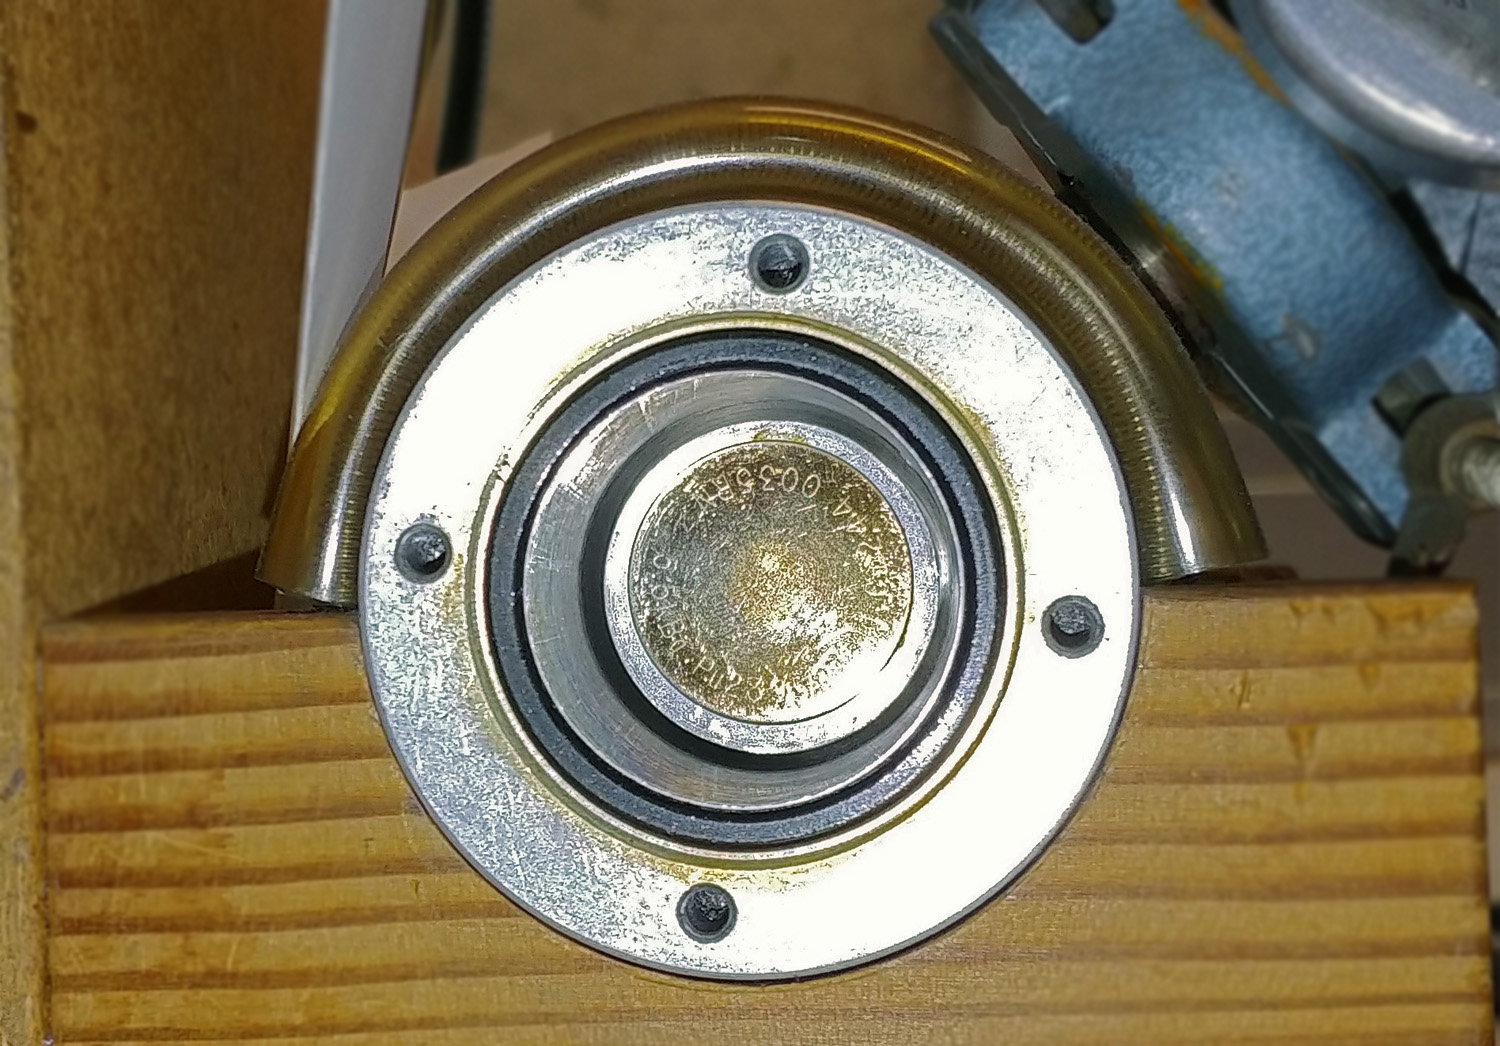
\includegraphics[width=\linewidth]{img/quelle_foto}}
	\caption{Interior views of the vacuum container.}
\end{figure}
\begin{figure}
	\centering
	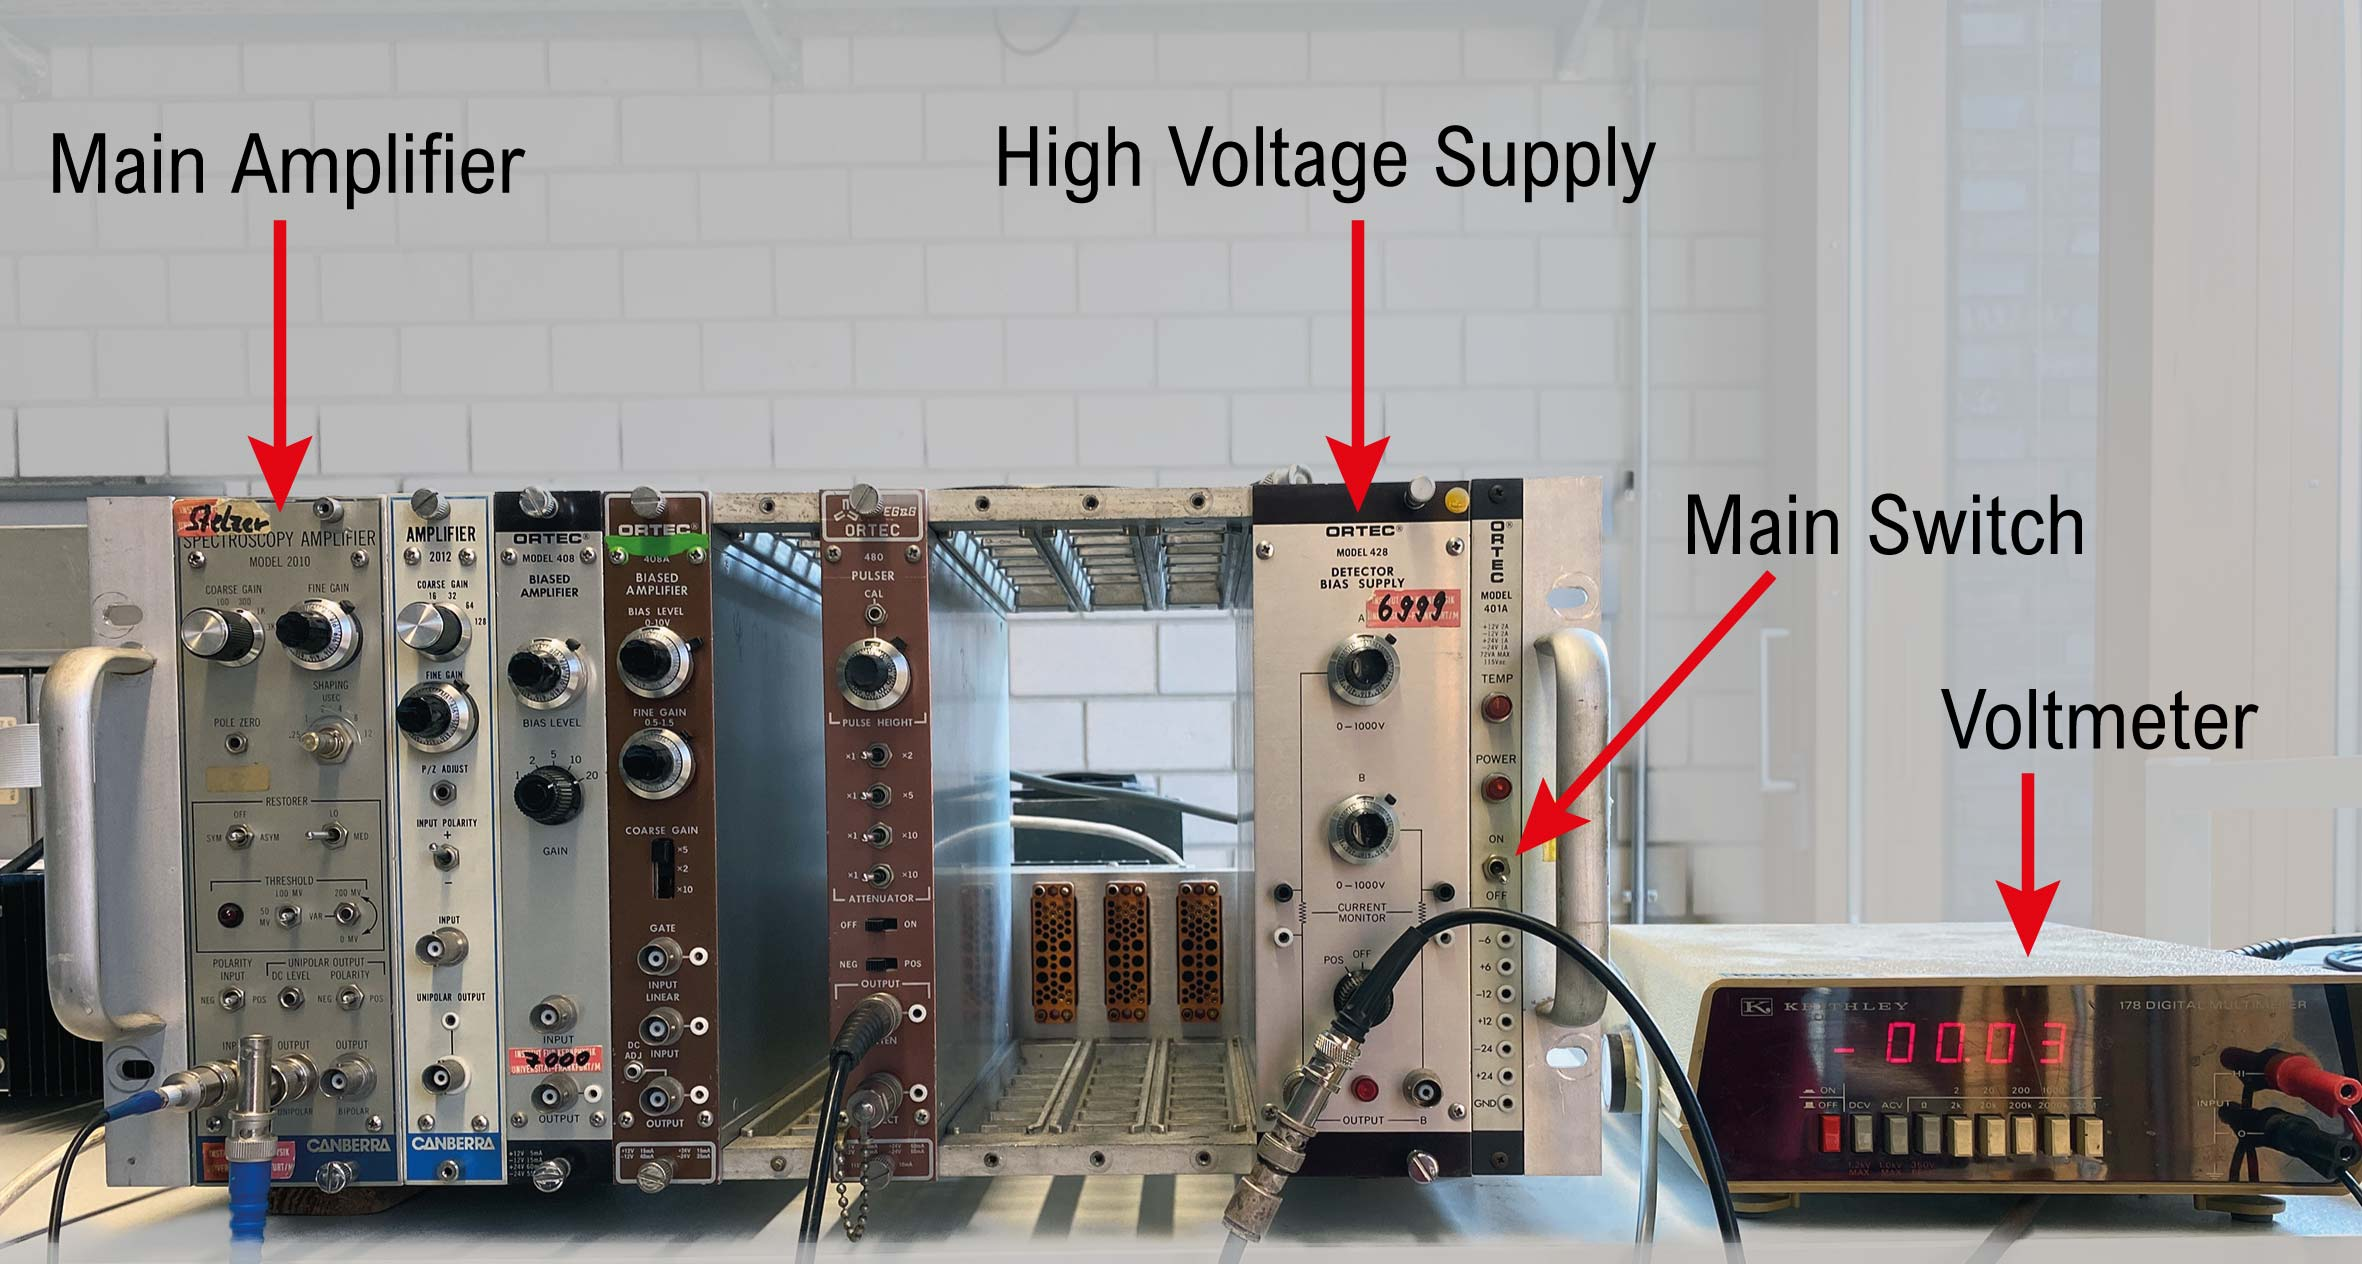
\includegraphics[width=0.75\linewidth]{img/setup_3.jpg}
	\caption{Electronics in the \enquote{Ortec-Crate}.}
	\label{fig:setup3}
\end{figure}

% !TeX spellcheck = en_US
\clearpage
\section{Experimental procedure and evaluation}
%
\subsection{Warning notices}\label{sec:warningnotices}
%
\begin{minipage}[c]{.15\linewidth}
	
\includegraphics[width=1.5cm]{img/toxic}
\end{minipage}
\begin{minipage}[t]{.85\linewidth}
	Eating and drinking is prohibited in the laboratory.
\end{minipage}\vspace{1em}\\ 
\begin{minipage}[c]{.15\linewidth}
	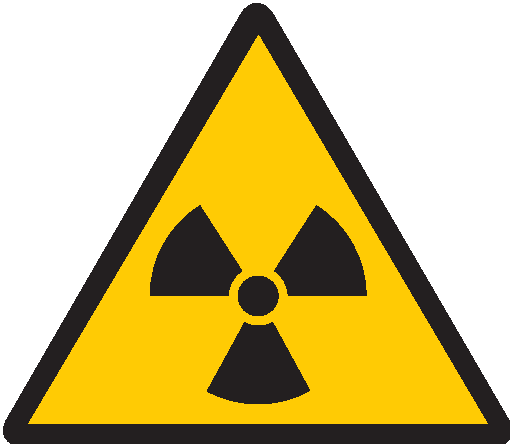
\includegraphics[width=1.5cm]{img/radioactive}
\end{minipage}
\begin{minipage}[t]{.85\linewidth}
	The radiation source used emits radioactive alpha radiation. It is weakly sealed and partially open. Radiation protection requires special safety measures for such sources. For this reason, the source has been permanently installed in the apparatus so that no radioactive material can escape from it into the room and no contact with the source is possible. Therefore, the measuring apparatus must not be opened under any circumstances. The ventilation valve should remain open for as short a time as possible.
\end{minipage}\vspace{1em}\\ 
\begin{minipage}[c]{.15\linewidth}
	
\includegraphics[width=1.5cm]{img/electric}
\end{minipage}
\begin{minipage}[t]{.85\linewidth}
	The maximum voltage on the semiconductor detector is $200$ V. Always change the voltage slowly. Exceeding the voltage can destroy the detector.
	\\ \\
	Only make changes to the wiring when the power supply is switched off.
	\\ \\
	The detector is extremely sensitive to light, operation with high voltage applied outside the closed vacuum chamber would destroy it.
\end{minipage}\vspace{1em}\\ 
\begin{minipage}[c]{.15\linewidth}
	
\includegraphics[width=1.5cm]{img/attention}
\end{minipage}
\begin{minipage}[t]{.85\linewidth}
	Do not open both venting valves of the vacuum piston at the same time.
	\\ \\
	Switch off the high voltage before venting.
\end{minipage}\vspace{1em}\\ 
%
\clearpage
%
\subsection{Preparations}
Go through this checklist together with the supervisor:
\begin{enumerate}
	\item Check the wiring (see Figure \ref{fig:verkabelung});
	\item Ensure that the power supply unit is set to $0$ V;
	\item Set the source to the smallest possible distance from the detector \\$r_{rel} = 0$ mm;
	\item Evacuate the vacuum chamber;
	\item Switch on Ortec-Crate;
	\item Start MCA3 Software on the PC.
\end{enumerate}
%
\subsection{Task 1: Saturation voltage}
The aim of the first task is to determine the saturation voltage of the semiconductor detector. The measurement is performed in vacuum at the smallest possible distance $r_{rel} = 0$ mm, and only for Plutonium.
\begin{enumerate}[label=\textbf{\alph*)}]
	\item At detector voltage $U_A = 0$ $V$, acquire a histogram with at least 8000 counts. Determine 
		\begin{itemize}[nosep]
		\item the peak position $\mu\ [\text{ADC Channels}]$;
		\item the half-width \textit{FWHM} [ADC Channels];
		\item and the counting rate $Z$ [1/s]
	\end{itemize}
	of the Plutonium peak using a Gaussian fit in the software.
	\item Repeat a) for the voltages $U_A = 8, 15, 20, 25, 30, 40, 70, 100$ V.
	\item Plot the peak position $\mu$, the count rate $Z$ and the percent resolution 
		\begin{equation}
			d_E = \frac{\textit{FWHM}}{\mu} \cdot 100 \qquad [\%]
		\end{equation}
	 as a function of $U_A$.
	\item Determine approximately the saturation voltage $U_{sat.}$ using the graphs. Select a voltage $U_{Det.}$ for your subsequent measurements. Explain your selection and the significance of the saturation voltage for using the semiconductor detector for $\alpha$-particle spectroscopy.
\end{enumerate}

\subsection{Task 2: Calibration and offset distance}
In this task, an energy calibration of the multi-channel analyzer is performed and the minimum adjustable distance $r_0$ (zero-distance) between detector and source is determined. The measurements take place in vacuum. 

\begin{enumerate}[label=\textbf{\alph*)}]
	\item Set the power supply voltage to the value $U_{Det.}$ determined in task 1;
	\item Record a reference spectrum with at least 12000 counts at $r_{rel} = 0$ mm.
		\\ Save a screenshot of the reference spectrum for your report.
		\\ \textit{Optional: } Save the histogram as a \texttt{.txt} file. This allows you to repeat the calibration at home.
	\item Calibrate the multi-channel analyzer in the software. To do this, determine the position of the three main maxima in the histogram by Gaussian fit and use the matching energies from Figure \ref{fig:schemata}. 
	
	Perform the Gaussian fits again to obtain the calibrated values for positions [keV], half-widths [keV] and count rates [1/s].
	\item Record at least 3000 counts at the relative distances $r_{rel} = 5, 10, 15, 20, 30$ mm and determine the calibrated positions, half-widths and count rates of the three main maxima by Gaussian fit.
	\item \textit{In the laboratory:} Plot the count rate as a function of the relative distance for Plutonium.
	
	\textit{In the report:} Plot the energy, percentage detector resolution and the counting-rate as a function of the relative distance for all isotopes.
	\item Determine the zero-distance $r_0$ between sample and detector in order to be able to use the effective distance $r_{eff} = r_0 + r_{rel}$ for the next measurements. To do this, consider how the distance law
	\begin{equation}
		Z \propto \frac{1}{r^2_{eff}},
	\end{equation}
	where $Z$ is the count rate in $[1/s]$, can be transformed and cleverly plotted to read the zero-distance directly from the y-axis intercept. Give the averaged result from the measurements of all three isotopes and present all values in a table.
 
    \textit{Note}: Looking at the error bars, decide wether to use the mean or the weighted mean with variance-defined weights to obtain the final result of $r_0$. See equation~\eqref{eq:weighted_mean} on page~\pageref{eq:weighted_mean} in the appendix.

\end{enumerate}
%
\subsection{Task 3: Range in air}
In the last part of the experiment, the differential energy loss of alpha radiation in air is determined.

\begin{enumerate}[label=\textbf{\alph*)}]
	\item Close the outlet valve of the vacuum chamber. Then slowly open the inlet valve until atmospheric pressure is established in the chamber. Then close the inlet valve again.
	\item Determine at $r_{rel} = 0, 4, 8, 20, 24, 28, 32, 36, \dots$ mm using a Gaussian fit:
	\begin{itemize}[nosep]
		\item the calibrated peak position $\mu\ [\text{keV}]$;
		\item the calibrated half-width \textit{FWHM} [keV];
		\item the count rate $Z$ [1/s];
	\end{itemize}
	for the main maxima of the three isotopes. If necessary, further increase the relative distance by $4$~mm per step until the plutonium signal disappears at $r_{max}$. Then take three additional measurements at $r_{rel} = r_{max} - 2, r_{max} - 6, r_{max} - 10$~mm. Record at least 2000 counts for each measurement.
	\item \textit{In the laboratory:} Plot the $\alpha$-energy $E\, \widehat{=}\, \mu$ depending on the effective distance for Plutonium. 
	
	\textit{In the report:} Plot the energy, the percentage resolution of the energy measurement, as well as the count rate depending on the effective distance for all three isotopes.
	\item Determine approximately -- by extrapolation with the eye -- the range of the $\alpha$-particles and their exit energy using the graph showing effective distance versus energy. What influences the uncertainty of the results the most?
	
	Compare the results with the literature values in a table. Use the given exit energies and Geiger's empirical range law, which gives the range $R$ [mm] depending on the exit energy $E_0$ [MeV] of the $\alpha$-particles:
	\begin{equation}\label{eq:geigerreachlaw}
		R = 3.1 \cdot \left(E_0\right)^{3/2}
	\end{equation}
	\textit{Optional:} If equation \ref{eq:geigerreachlaw} is transformed and adjusted accordingly, it is suitable as a fit function for the data. This allows range and exit energy to be determined more accurately than can be determined by eye.
	\item \textit{In the laboratory:} Plot the differential energy loss as a function of the effective distance $\left( \Delta E/ \Delta x \ \text{vs.}\ r_{eff} \right)$ for Plutonium.
	
	\textit{In the report:} Add the Bragg-Peaks of the other isotopes. Give an estimate of the maximum value of the energy loss and an estimate of the energy loss close to the sample. Compare the three Bragg curves with each other.
	\item Estimate the different contributions that go into the energy resolution. Consider the detector resolution from the vacuum and air measurements. Discuss the significance of the electronic noise, the statistical fluctuations in the number of electron-hole pairs (Fano factor), as well as the finite thickness of the source and the energy straggling.
\end{enumerate}


\newpage
\appendix
%
\section{Appendix}\label{sec:appendix}
%
\subsection{Your Report}
Together with the report, submit your original measurement data as a neat \texttt{.txt}-file with appropriate comments so that the data can be assigned to the respective measurements. The structure of the protocol should be based on the following points:
\begin{itemize}
	\item Theory section
	\item Execution and evaluation
	\begin{itemize}
		\item What is to be measured and why?
		\item What measurement results are expected?
		\item How is the measurement carried out?
		\item What was actually measured? How large are the measurement errors?
		\item What can be learned from the measurement result? Were the expectations met?
		What are the sources of error?
	\end{itemize}
	\item Conclusion
\end{itemize}
%
\subsubsection*{Error Handling}
All data in your diagrams should be displayed with both x and y error bars.
When carrying out the experiment, you will already receive the standard deviations for the measured values from the Gaussian fits. 
You can make sensible assumptions about the uncertainties of the other measured values. 
Create tables with measured values and associated uncertainties and explicitly state the formulas used for the calculation.
For variables that are calculated from several (error-prone) measured values, carry out Gaussian error propagation:
\begin{equation}\label{eq:RSS}
	\sigma_{f} = \sqrt{\left( \frac{\partial f}{\partial x_1}\ \sigma_{x_1} \right)^2 + \left( \frac{\partial f}{\partial x_2}\ \sigma_{x_2} \right)^2 + ... + \left( \frac{\partial f}{\partial x_n}\ \sigma_{x_n} \right)^2} 
\end{equation}
Here, $\sigma_{f}$ is the uncertainty of the quantity $f = f (x_1, x_2, ... , x_n)$, which is dependent of the measured values $x_1, x_2, ... , x_n$ and their respective uncertainties $\sigma_{x_1}, \sigma_{x_2}, ..., \sigma_{x_n}$. 

Alternatively, estimate the maximum error limits with
\begin{equation}\label{eq:abs}
		\sigma_{f} = \left| \frac{\partial f}{\partial x1}\right| \sigma_{x1} + \left| \frac{\partial f}{\partial x2}\right| \sigma_{x2} + ... + \left| \frac{\partial f}{\partial xn}\right| \sigma_{xn}
\end{equation}
%
\subsection{Notes}
%
\subsubsection*{Weighted Mean}
The weighted mean $\overline{x}$ of several measured values $x_i$ of the same quantity $x$ is defined as
\begin{subequations}\label{eq:weighted_mean}
    \begin{align}
    \overline{x} & = \frac{\sum\limits_{i}\ w_i \ x_{i}}{\sum\limits_{i} \ w_i }  \label{eq:wmean}\\
    \text{with weights } \quad w_i & = (\Delta x_{i})^{-2} \\
    \text{and error } \quad \Delta \overline{x} & = \left(  \sum\limits_{i} w_i  \right)^{-\frac{1}{2}} \label{eq:wmeanerr}
    \end{align}
\end{subequations}
here, $\Delta x_i$ is the uncertainty of the $i$-th single measurement value.


\clearpage
\begin{thebibliography}{1}
	\bibitem{kolanoski} 
	Kolanoski, H., Wermes, N., 2016. \emph{Particle Detectors}. Springer-Verlag Berlin Heidelberg. \textsc{doi:} \url{https://doi.org/10.1007/978-3-662-45350-6} (German version).
	
	\bibitem{povh-rith}
	Povh, B., Rith, K. u.a., 2015. \emph{Particles and Nuclei}. Springer-Verlag Berlin Heidelberg. \textsc{doi:} \url{https://doi.org/10.1007/978-3-662-46321-5}
	
	\bibitem{leo}
	Leo, W.R., 1994. \emph{Techniques for Nuclear and Particle Physics Experiments: A How-To Approach}. Springer Berlin / Heidelberg. ISBN 9783642579202. 
	
	\bibitem{pdg}
	Particle Data Group, Workman, R. L. u.a., 2022, \emph{Review of Particle Physics}, \textsc{in:} Progress of Theoretical and Experimental Physics 2022, Issue 8, 083C01, \textsc{doi:} \url{https://doi.org/10.1093/ptep/ptac097}
	
	\bibitem{NDS2014} % Quelle für Energien von Plutonium
	Browne, E., Tuli, J.K. 2014. Nuclear Data Sheets 122, 205 (2014). \url{https://www.nndc.bnl.gov/nudat3/decaysearchdirect.jsp?nuc=239Pu&unc=NDS}
	
	\bibitem{NDS2006} % Quelle für Energien von Americium
	Basunia, M.S., 2006. Nuclear Data Sheets 107, 3323 (2006). \url{https://www.nndc.bnl.gov/nudat3/decaysearchdirect.jsp?nuc=241Am&unc=NDS}
	
	\bibitem{NDS2008} % Quelle für Energien von Curium
	Singh, B., Browne, E., 2008. Nuclear Data Sheets 109, 2439 (2008). \url{https://www.nndc.bnl.gov/nudat3/decaysearchdirect.jsp?nuc=244Cm&unc=NDS}

	\bibitem{bleck-neuhaus}
	Bleck-Neuhaus, J., 2013. \emph{Elementare Teilchen: Von den Atomen über das Standard-Modell bis zum Higgs-Boson}. Springer-Verlag Berlin Heidelberg. 2. Aufl. \textsc{doi:} \url{https://doi.org/10.1007/978-3-642-32579-3}
	
	\bibitem{dewiki:240085809}
	Wikipedia, 2023, \emph{Alphastrahlung}, \url{https://de.wikipedia.org/w/index.php?title=Alphastrahlung&oldid=240085809},
	[Online; Stand 5. März 2024]
	
	\bibitem{img:coulombwall}
	Johannes Schneider, CC BY-SA 4.0, \url{ https://commons.wikimedia.org/w/index.php?curid=61182444}
\end{thebibliography}


	
\end{document}